\documentclass[12pt, oneside]{report}
\usepackage{geometry}
\geometry{a4paper,top=3cm,bottom=3cm,left=3cm,right=3cm,heightrounded}
\usepackage[english]{babel}
\usepackage[utf8x]{inputenc}
\usepackage{amsmath, amsthm, amssymb}
\usepackage{graphicx}
\usepackage{siunitx}
\usepackage[table]{xcolor}% http://ctan.org/pkg/xcolor
\usepackage{units}
\usepackage{verbatim} 
\usepackage{color}
\usepackage{subcaption} 
\usepackage{pdflscape}
\usepackage{bm}
\usepackage{tabularx}
\usepackage{array}
\usepackage{epstopdf}
\usepackage{listings}
\usepackage{multirow}
\usepackage{eurosym}
\usepackage{booktabs}
\usepackage{longtable}
\usepackage{caption}
\usepackage{enumitem}
\usepackage{hyperref}
\usepackage{tablefootnote}
\usepackage{setspace}
\usepackage{quoting}
\usepackage{wrapfig}
\usepackage{times}
\usepackage{fancyhdr}
\usepackage{url}
\usepackage{titlesec}
\lstset{language=Matlab,%
	basicstyle=\small\ttfamily,
	numbers=left,
	numberstyle=\tiny,
	stepnumber=2,
	frame=lines
}


\setlength\parindent{0pt} % Removes all indentation from paragraphs
%\hypersetup{
%	colorlinks=true,
%	urlcolor=black,
%	linkcolor=black,
%	pdftitle={Micro e nano system},
%	bookmarks=true}
\usepackage{eso-pic}

\def\nicefrac#1#2{\leavevmode%
	\raise.5ex\hbox{\small #1}%
	\kern-.1em/\kern-.15em%
	\lower.25ex\hbox{\small #2}}

	\newcommand{\ohm}{$\Omega$\ }
	\newcommand{\micro}{\textmu}
	
	\usepackage{eso-pic}
	

\begin{document}
	\renewcommand{\chaptername}{Chapter}

	\begin{titlepage}
	
	\newcommand{\HRule}{\rule{\linewidth}{0.5mm}} % Defines a new command for the horizontal lines, change thickness here
	
	\center % Center everything on the page
	
	%----------------------------------------------------------------------------------------
	%	LOGO SECTION
	%----------------------------------------------------------------------------------------
	
	
\includegraphics[height=7cm]{immagini/polito.png}\\[0.5cm] % Include a department/university logo - this will require the graphicx package
	
	%----------------------------------------------------------------------------------------
	%	HEADING SECTIONS
	%----------------------------------------------------------------------------------------
	
	{\LARGE Politecnico di Torino}\\[0.8cm] % Name of your university/college
	\HRule \\[1cm]
	%\emph{{\LARGE Master of Science on Electronic Engineering and Nanotechnologies for ICTs}}\\[0.3cm]

	{\huge\LARGE Integrated Systems Technology}\\[0.5cm] % Major heading such as course name
	\emph{{prof. Gianluca Piccinini}}\\
	\emph{{prof. Marco Vacca}}\\[0.5cm] % Minor heading such as course title
	
	
	%----------------------------------------------------------------------------------------
	%	TITLE SECTION
	%----------------------------------------------------------------------------------------
	
	\HRule \\[1cm]
	{ \Huge \textsf{Modelling of Multiplexers}}\\[0.5cm] % Title of your document
	\HRule \\[1cm]
	\textit{{\large {Group 8}}}\\[0.4cm]
	
	\begin{center}
		\begin{table}[ht]\centering%\caption{}
			\begin{tabular}{c|c}
				\hline
				\textit{Authors}&\textit{student ID}\\ \hline
				Jacopo Acquafresca&232417\\ \hline
				Carlo Alberto Cristofanini&224689\\ \hline
				Marco Guerra&231317\\ \hline
				Lorenzo Mairone&228293\\ \hline
				
				
			\end{tabular}
			\label{tab:3}
		\end{table}
	\end{center}
	\emph{{\large Academic year 2016/2017}}\\[0.5cm] % Minor heading such as course title
	%----------------------------------------------------------------------------------------
	%	DATE SECTION
	%----------------------------------------------------------------------------------------
	%----------------------------------------------------------------------------------------
	\vfill % Fill the rest of the page with whitespace
	\thispagestyle{empty}
\end{titlepage}
	
\begingroup 
\makeatletter\let\ps@plain\ps@empty\makeatother 
\tableofcontents
\thispagestyle{empty} % elimino il numero di pagina nell'indice
\cleardoublepage 
\thispagestyle{empty} % elimino il numero di pagina nell'indice
\endgroup

	 


	%\singlespacing
	\onehalfspace % interlinea 1.5
	%\doublespacing
	
	%\cleardoublepage
	\quotingsetup{font=small}

	\pagestyle{fancy}
	\fancyhf{} % azzeriamo i campi
	\fancyhead[RE]{\leftmark}
	\fancyhead[LO]{\nouppercase{\rightmark}}	
	\pagenumbering{arabic}
	\fancyfoot[C]{\thepage}	
	
	%inserire qui tutti i capitoli
	\chapter{Introduction}
Aim of this project is to carry out a comparative analysis at system level between different typology of CMOS multiplexers. We will perform several evaluations concerning the static and dynamic power consumption, the occupied area and time delay in different digital circuit configurations, within 2010 HP, LOP and LSTP technologies. Physical constants, system parameters and technological variables have been taken from TAMTAMS, a useful tool allowing to predict system level features starting from technology variables. In this project we will present multiplexer circuits built with NAND gates, enabling a fast and interesting analysis of the performances.

\section{Multiplexer architecture}
The multiplexer (\ref{mux_blocchi}) is a combinational logic circuit designed to switch several input lines toward a single common output line by the application of a control signal.\\
\begin{figure}[!h]
	\centering
	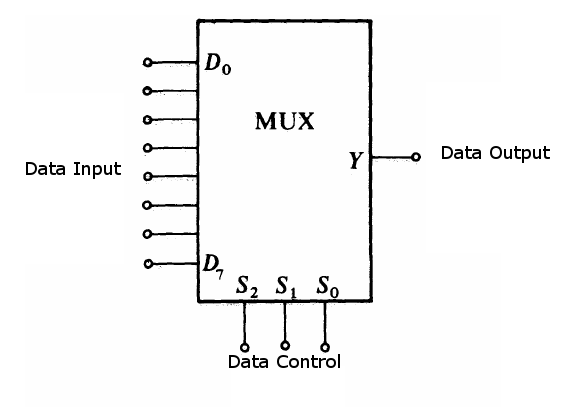
\includegraphics[scale=0.5]{immagini/mux_blocchi.png}
	\caption{\textit{Multiplexer block diagram.}} 
	\label{mux_blocchi}
\end{figure}
\newline
Multiplexers can be either digital circuits made from high speed logic gates used to switch digital or binary data.
In digital electronics, multiplexers are also known as data selectors because they can “select” among different input lines.
They are used as a method to reduce number of data lines required in a circuit design or when a single data line or data bus is used to transfer two or more different digital signals.\\
Generally, the selection of each input line in a multiplexer is controlled by an additional set of inputs called control lines, and according to the binary condition of these control inputs, either “high” or “low”, the appropriate data input is connected directly to the output.\\
Normally, a multiplexer has an even number of ($2^N$) data input lines with $N$ selection inputs.\\
In figure \ref{mux_funz} is shown the logic circuit of the simplest multiplexer unit next to his truth table. When the selection input is \textit{S = 0}, the upper AND gate is selected (\textit{G0}) and the digital data (0 or 1) present at the input data \textit{D0} is transferred to the output. Conversely when \textit{S = 1}, the upper AND gate is enabled (\textit{G1}) and the value \textit{D1} it is transferred at the output. The logic function that expresses the output is
\begin{equation}
Y=D_0\bar S+D_1S.
\label{eq1}
\end{equation}
\begin{figure}[!h]
	\centering
	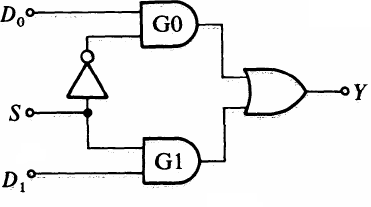
\includegraphics[scale=0.6]{immagini/mux_1.png}
	\caption{\textit{Logic circuit implementation of a multiplexer with two inputs.}} 
	\label{mux_1}
\end{figure}

\begin{figure}[!h]
	\centering
	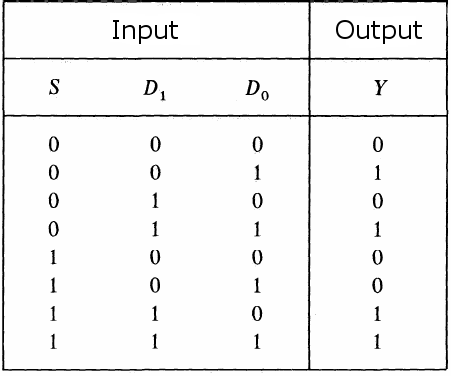
\includegraphics[scale=0.4]{immagini/mux_fun1.png}
	\caption{\textit{Truth table.}} 
	\label{mux_funz}
\end{figure}
\newpage
\section{Multiplexer with NAND gates}
In principle, any combinatorial logic function can be realized with enough NAND gates through the two De Morgan theorems:
\begin{equation}
\overline{A\cdot B}= \overline{A} + \overline{B}
\label{de1}
\end{equation}
\begin{equation}
\overline{A + B}= \overline{A} \cdot \overline{B}
\label{de2}
\end{equation}
The first \ref{de1} one mentions that the negated product of two variables is equal to the sum of negated variables.\\
The second \ref{de2} theorem is stating that the negated sum of two variables is equal to the product of the single negated variables.\\
Applying to the figure \ref{mux_1} the De Morgan's theorems allows to redefine the entire circuit using only NAND gates.
\begin{equation}
Y=\overline{\overline{D_0 + \overline{S + S}}+\overline{D_1+S}}
\label{de3}
\end{equation}
\begin{figure}[!h]
	\centering
	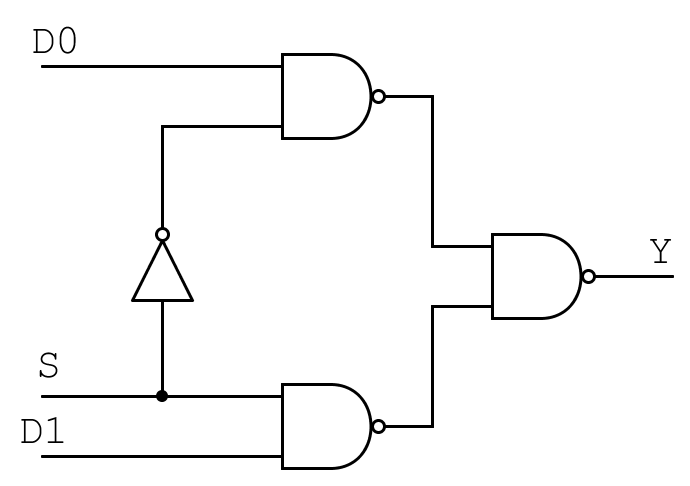
\includegraphics[scale=0.5]{immagini/mux_3.png}
	\caption{\textit{Circuit implementation of a multiplexer with two inputs optimized.}} 
	\label{mux_2}
\end{figure}
\newline
The inverter can be easily imagined as a NAND port with the inputs connected together.
\begin{figure}[!h]
	\centering
	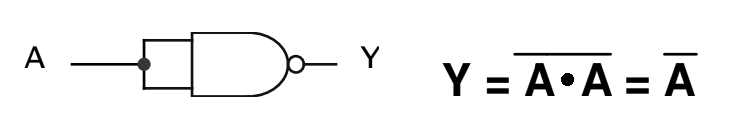
\includegraphics[scale=0.6]{immagini/not_nand.png}
	\caption{\textit{Inverter made with a NAND}} 
	\label{not}
\end{figure}
\newline
By implementing these properties the logical scheme becomes:
\begin{figure}[!h]
	\centering
	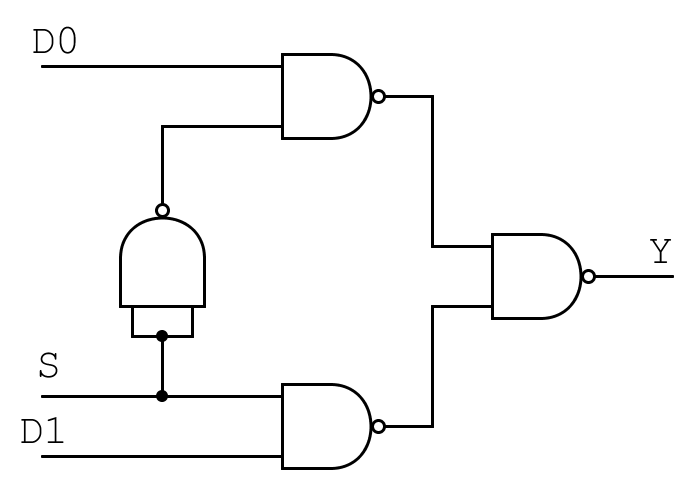
\includegraphics[scale=0.4]{immagini/2_to_1_1bit}
	\caption{\textit{Circuit implementation of a  multiplexer 2 to 1 with only NAND gates.}} 
	\label{2_to_1_1bit}
\end{figure}
We choose to use basic NAND configurations as they allow a simpler approach, namely to evaluate the area and power consumption of a single NAND gate and multiply it by the number of those that make up the circuit.\\ With a single 2 to 1 mux unit is possible to build more complex multiplexers, showing a tree circuit structure. In figure \ref{8_to_1_1bit} is reported a multiplexer 8 to 1  with a word of 1 bit, using 24 NAND gates.
\begin{figure}[!h]
	\centering
	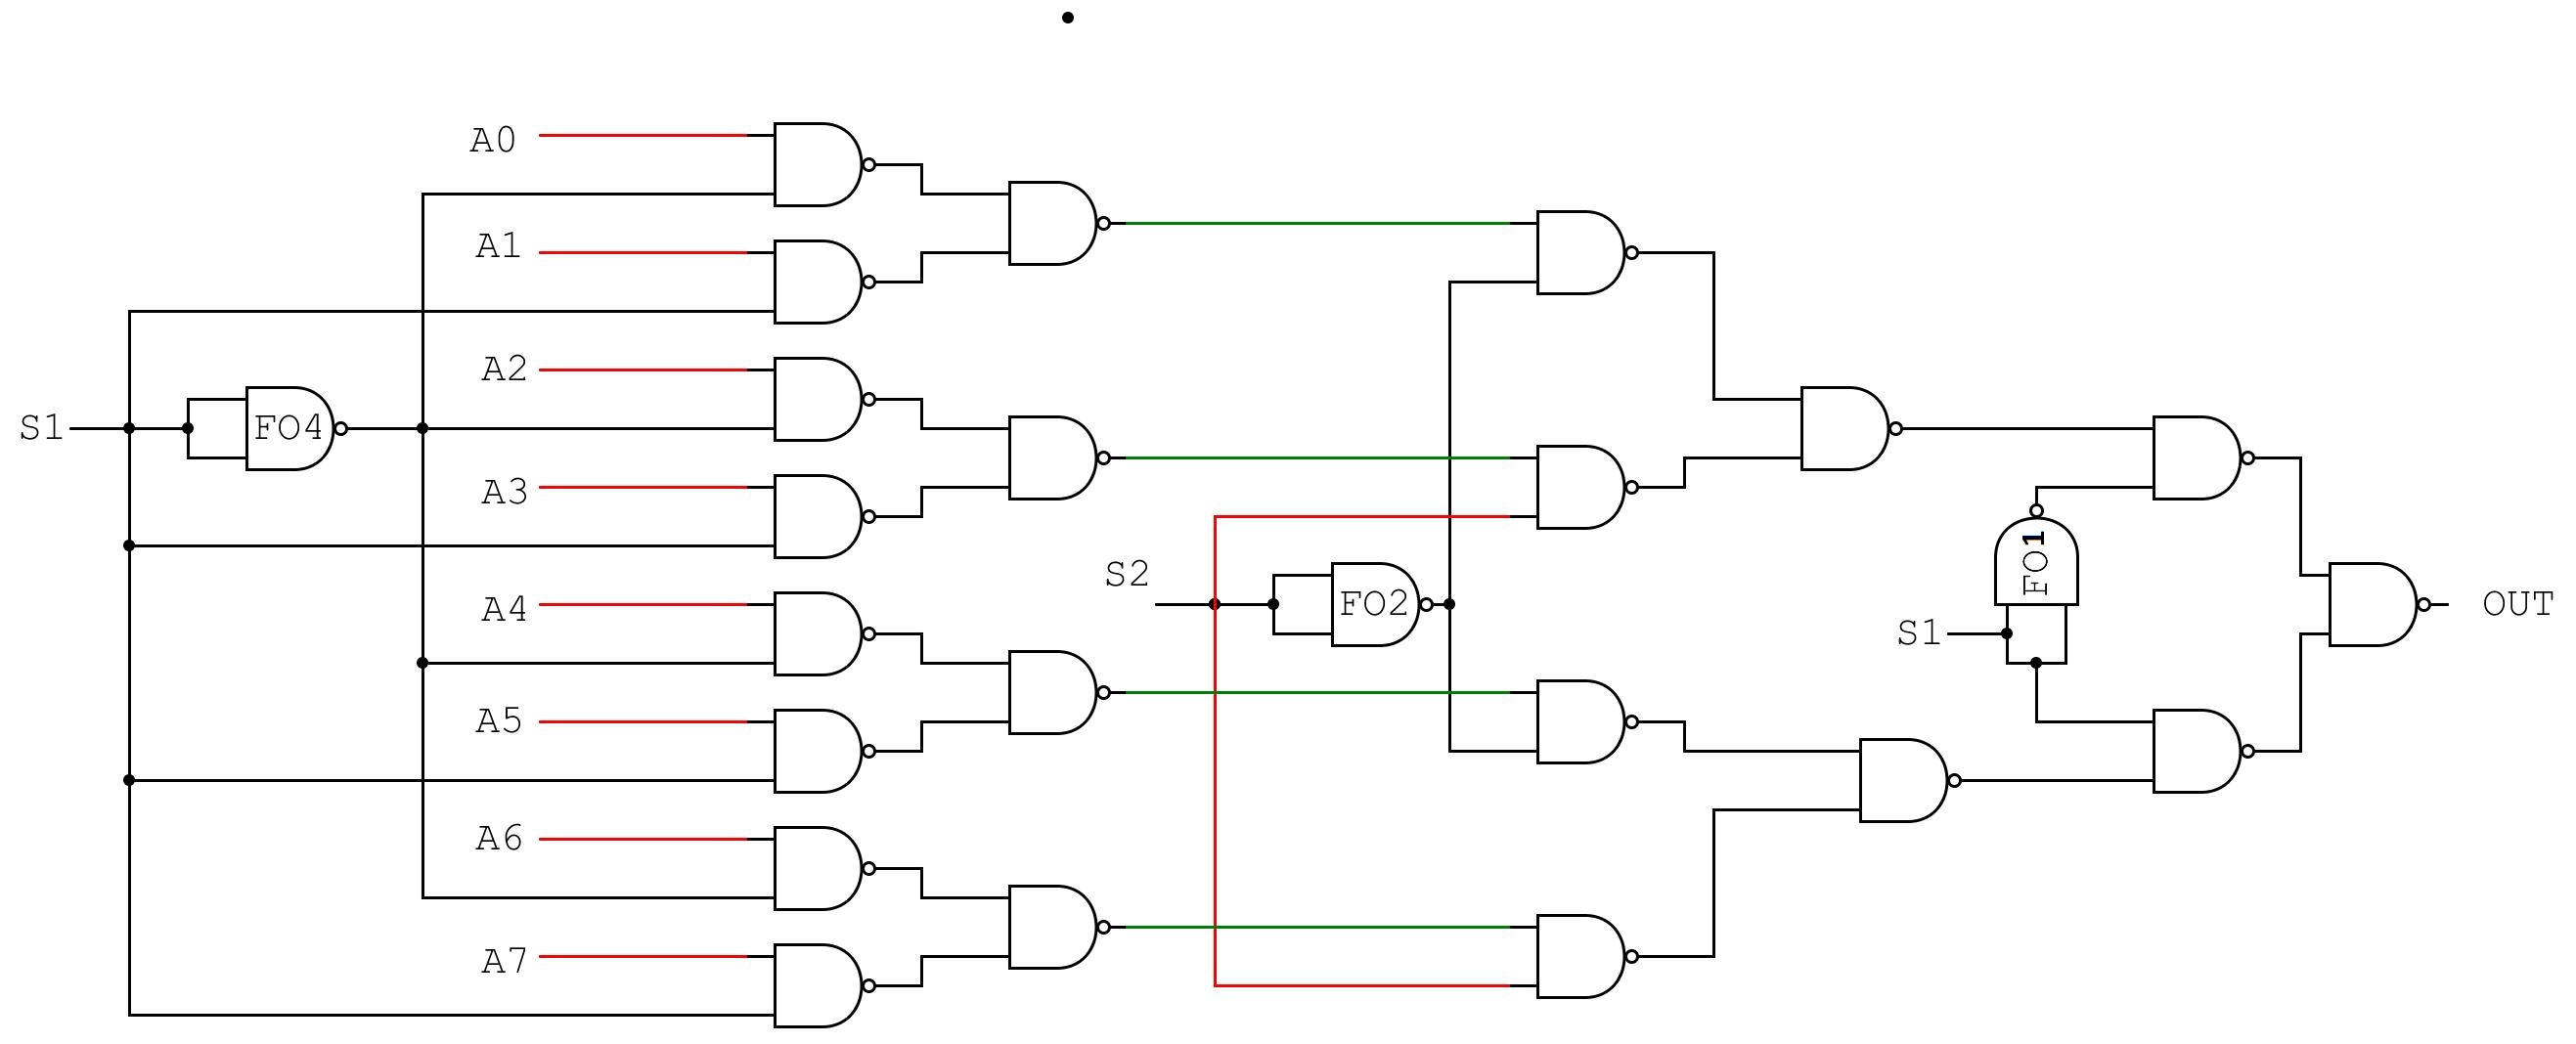
\includegraphics[scale=0.15]{immagini/8_to_1_1bit}
	\caption{\textit{Circuit implementation of a  multiplexer 8 to 1 with only NAND gates.}} 
	\label{8_to_1_1bit}
\end{figure}
\newpage
\section{CMOS realization of multiplexers} 
The next step is to realize a MUX circuit with transistors, by implementing CMOS technology. The building unit is reported in figure \ref{nand2} where a NAND gate is showed.
\begin{figure}[!h]
	\centering
	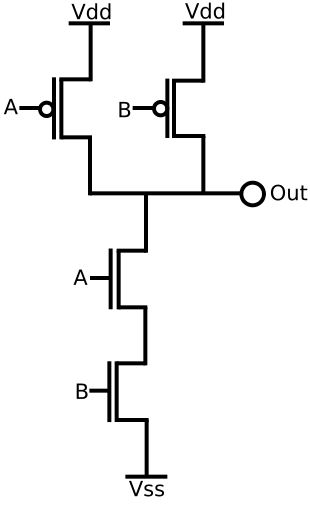
\includegraphics[scale=0.3]{immagini/nand2.png}
	\caption{\textit{CMOS circuit for a NAND gate.}} 
	\label{nand2}
\end{figure}
\newline
An example of CMOS multiplexer realization is reported in the figure below.
\begin{figure}[!]
	\centering
	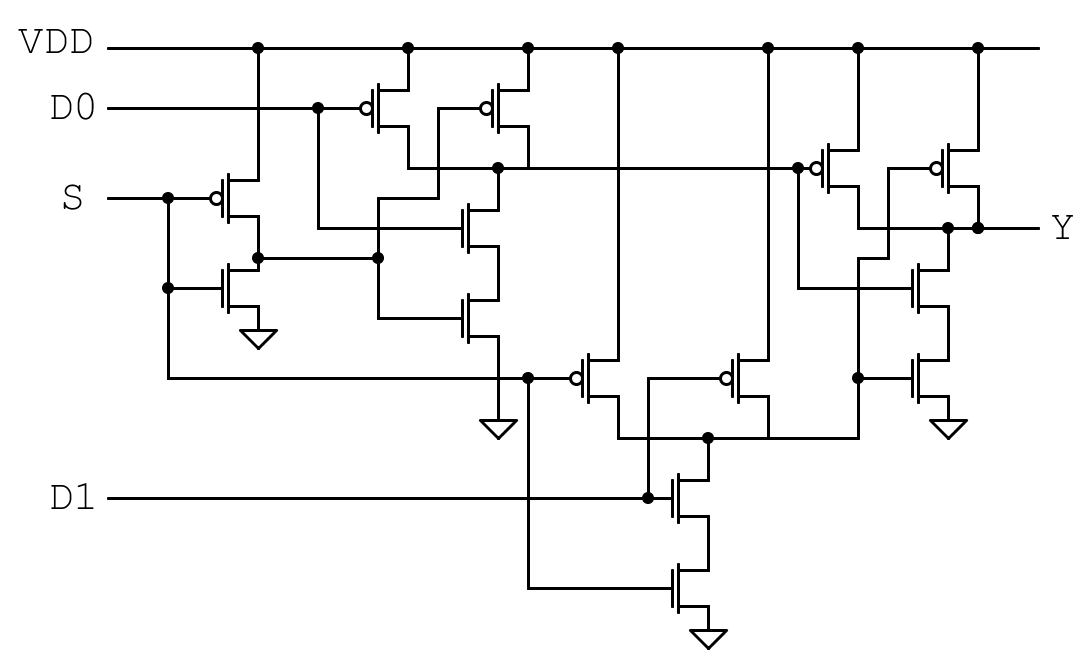
\includegraphics[scale=0.22]{immagini/trans}
	\caption{\textit{CMOS realization of a MUX 2x1.}} 
	\label{mux_3}
\end{figure}

\newpage
\section{Types of Multiplexer}
Here are summarized the different typologies of mutiplexer analysed. The various multiplexers vary by the number of input signals and the parallelism. 
\begin{itemize}\itemsep1pt
	\item Multiplexer 2 to 1 parallelism 16 bit
	\item Multiplexer 2 to 1 parallelism 32 bit
	\item Multiplexer 2 to 1 parallelism 64 bit 
	\item Multiplexer 8 to 1 parallelism 8 bit 	
	\item Multiplexer 16 to 1 parallelism 8 bit
	\item Multiplexer 16 to 1 parallelism 16 bit
	\item Multiplexer 16 to 1 parallelism 32 bit
	\item Multiplexer 16 to 1 parallelism 64 bit 
	\item Multiplexer 32 to 1 parallelism 8 bit
	\item Multiplexer 32 to 1 parallelism 16 bit
	\item Multiplexer 32 to 1 parallelism 32 bit
	\item Multiplexer 32 to 1 parallelism 64 bit 
	\item Multiplexer 64 to 1 parallelism 8 bit
	\item Multiplexer 64 to 1 parallelism 16 bit
	\item Multiplexer 64 to 1 parallelism 32 bit
	\item Multiplexer 64 to 1 parallelism 64 bit 
	\item Multiplexer 128 to 1 parallelism 8 bit
	\item Multiplexer 128 to 1 parallelism 16 bit
	\item Multiplexer 128 to 1 parallelism 32 bit
	\item Multiplexer 128 to 1 parallelism 64 bit 
\end{itemize}
\newpage
\section{NAND with TAMTAMS}
By using the application TAMTAMS web, it was possible to make a first analysis at system level of several parameters concerning CMOS NAND2 gates employed.  The input data used for the analysis are:
\begin{itemize}
	\item Year:\quad 2010;
	\item Technology branch:\quad HP, LOP, LSTP;
	\item model used for $I_{gate}$:\quad Mastar4.
\end{itemize}
From the analysis done we've obtained the following results:
\lstinputlisting{capitoli/code/HP_2010.m}	
%https://tamtams.vlsilab.polito.it/Documentation/TechnologyHTML/bulk/HP2010_dev_bul.html
\lstinputlisting{capitoli/code/LOP_2010.m}	%https://tamtams.vlsilab.polito.it/Documentation/TechnologyHTML/bulk/LOP2010_dev_bul.html
\lstinputlisting{capitoli/code/LSTP_2010.m}	%https://tamtams.vlsilab.polito.it/Documentation/TechnologyHTML/bulk/LSTP2010_dev_bul.html
As can be seen from the previous analysis, different fan out type of NAND2 are available with the respective values of static and dynamic power consumption. This will allow us to built our multiplexers by using different type of gates, reducing the overall occupation area. In particular, to build our multiplexers, we will use NAND gates with fan-out equal to 1, 2 and 4. 


%	\chapter{Multiplexer Architecture}
\section{General Description}
The multiplexer (\ref{mux_blocchi}) is a combinational logic circuit designed to switch several input lines toward a single common output line by the application of a control signal.\\
\begin{figure}[!h]
	\centering
	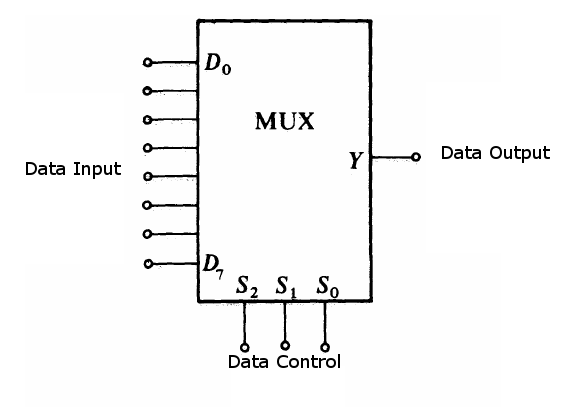
\includegraphics[scale=0.5]{immagini/mux_blocchi.png}
	\caption{\textit{Multiplexer block diagram.}} 
	\label{mux_blocchi}
\end{figure}
\newline
Multiplexers can be either digital circuits made from high speed logic gates used to switch digital or binary data.
In digital electronics, multiplexers are also known as data selectors because they can “select” among different input lines.
They are used as a method to reduce number of data lines required in a circuit design or when a single data line or data bus is used to transfer two or more different digital signals.\\
Generally, the selection of each input line in a multiplexer is controlled by an additional set of inputs called control lines, and according to the binary condition of these control inputs, either “high” or “low”, the appropriate data input is connected directly to the output.\\
Normally, a multiplexer has an even number of ($2^N$) data input lines with $N$ selection inputs.\\
In figure \ref{mux_funz} is shown the logic circuit of the simplest multiplexer unit next to his truth table. When the selection input is \textit{S = 0}, the upper AND gate is selected (\textit{G0}) and the digital data (0 or 1) present at the input data \textit{D0} is transferred to the output. Conversely when \textit{S = 1}, the upper AND gate is enabled (\textit{G1}) and the value \textit{D1} it is transferred at the output. The logic function that expresses the output is
\begin{equation}
Y=D_0\bar S+D_1S.
\label{eq1}
\end{equation}
\begin{figure}[!h]
	\centering
	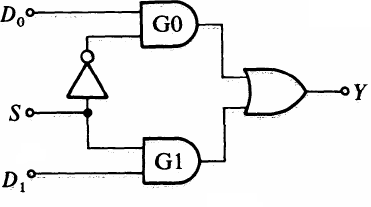
\includegraphics[scale=0.6]{immagini/mux_1.png}
	\caption{\textit{Logic circuit implementation of a multiplexer with two inputs.}} 
	\label{mux_1}
\end{figure}

\begin{figure}[!h]
	\centering
	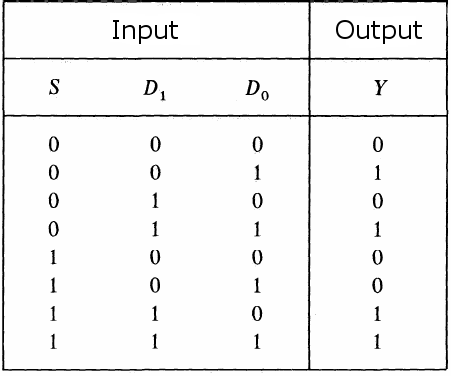
\includegraphics[scale=0.4]{immagini/mux_fun1.png}
	\caption{\textit{Truth table.}} 
	\label{mux_funz}
\end{figure}
\newpage
\section{Multiplexer with NAND gates}
In principle, any combinatorial logic function can be realized with enough NAND gates through the two De Morgan theorems:
\begin{equation}
\overline{A\cdot B}= \overline{A} + \overline{B}
\label{de1}
\end{equation}
\begin{equation}
\overline{A + B}= \overline{A} \cdot \overline{B}
\label{de2}
\end{equation}
The first \ref{de1} one mentions that the negated product of two variables is equal to the sum of negated variables.\\
The second \ref{de2} theorem is stating that the negated sum of two variables is equal to the product of the single negated variables.\\
Applying to the figure \ref{mux_1} the De Morgan's theorems allows to redefine the entire circuit using only NAND gates.
\begin{equation}
Y=\overline{\overline{D_0 + \overline{S + S}}+\overline{D_1+S}}
\label{de3}
\end{equation}
\begin{figure}[!h]
	\centering
	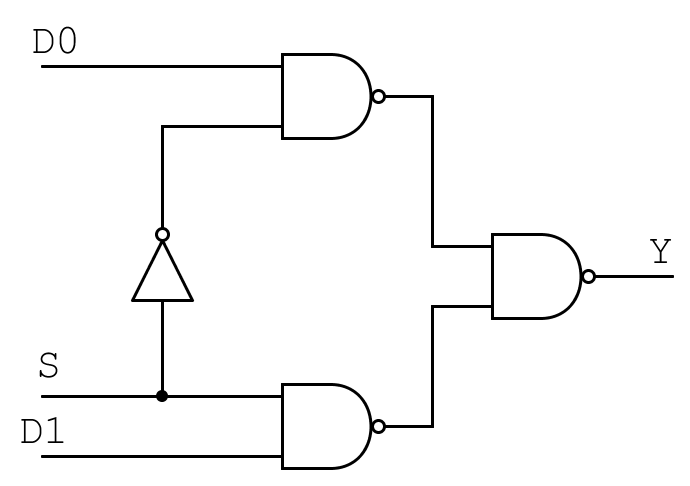
\includegraphics[scale=0.5]{immagini/mux_3.png}
	\caption{\textit{Circuit implementation of a multiplexer with two inputs optimized.}} 
	\label{mux_2}
\end{figure}
\newline
The inverter can be easily imagined as a NAND port with the inputs connected together.
\begin{figure}[!h]
	\centering
	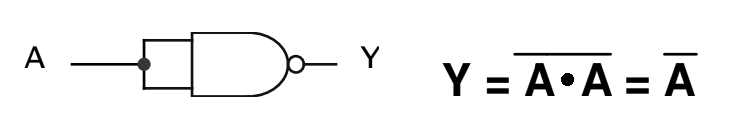
\includegraphics[scale=0.6]{immagini/not_nand.png}
	\caption{\textit{Inverter made with a NAND}} 
	\label{not}
\end{figure}
\newline
By implementing these properties the logical scheme becomes:
\begin{figure}[!h]
	\centering
	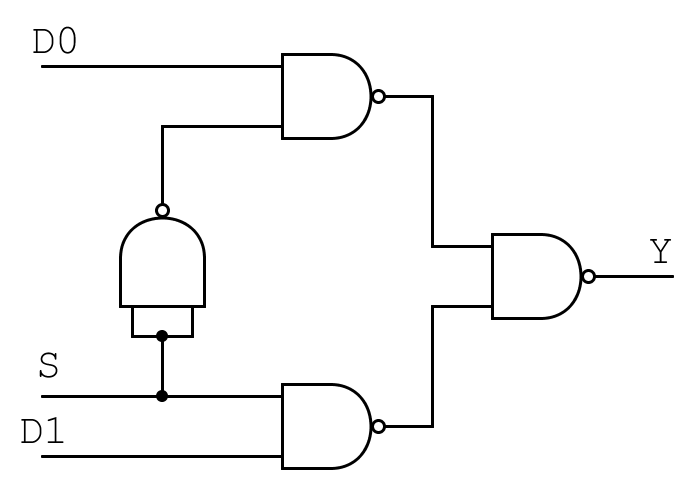
\includegraphics[scale=0.4]{immagini/2_to_1_1bit}
	\caption{\textit{Circuit implementation of a  multiplexer 2 to 1 with only NAND gates.}} 
	\label{2_to_1_1bit}
\end{figure}
We choose to use basic NAND configurations as they allow a simpler approach, namely to evaluate the area and power consumption of a single NAND gate and multiply it by the number of those that make up the circuit.\\ With a single 2 to 1 mux unit is possible to build more complex multiplexers, showing a tree circuit structure. In figure \ref{8_to_1_1bit} is reported a multiplexer 8 to 1  with a word of 1 bit, using 24 NAND gates.
\begin{figure}[!h]
	\centering
	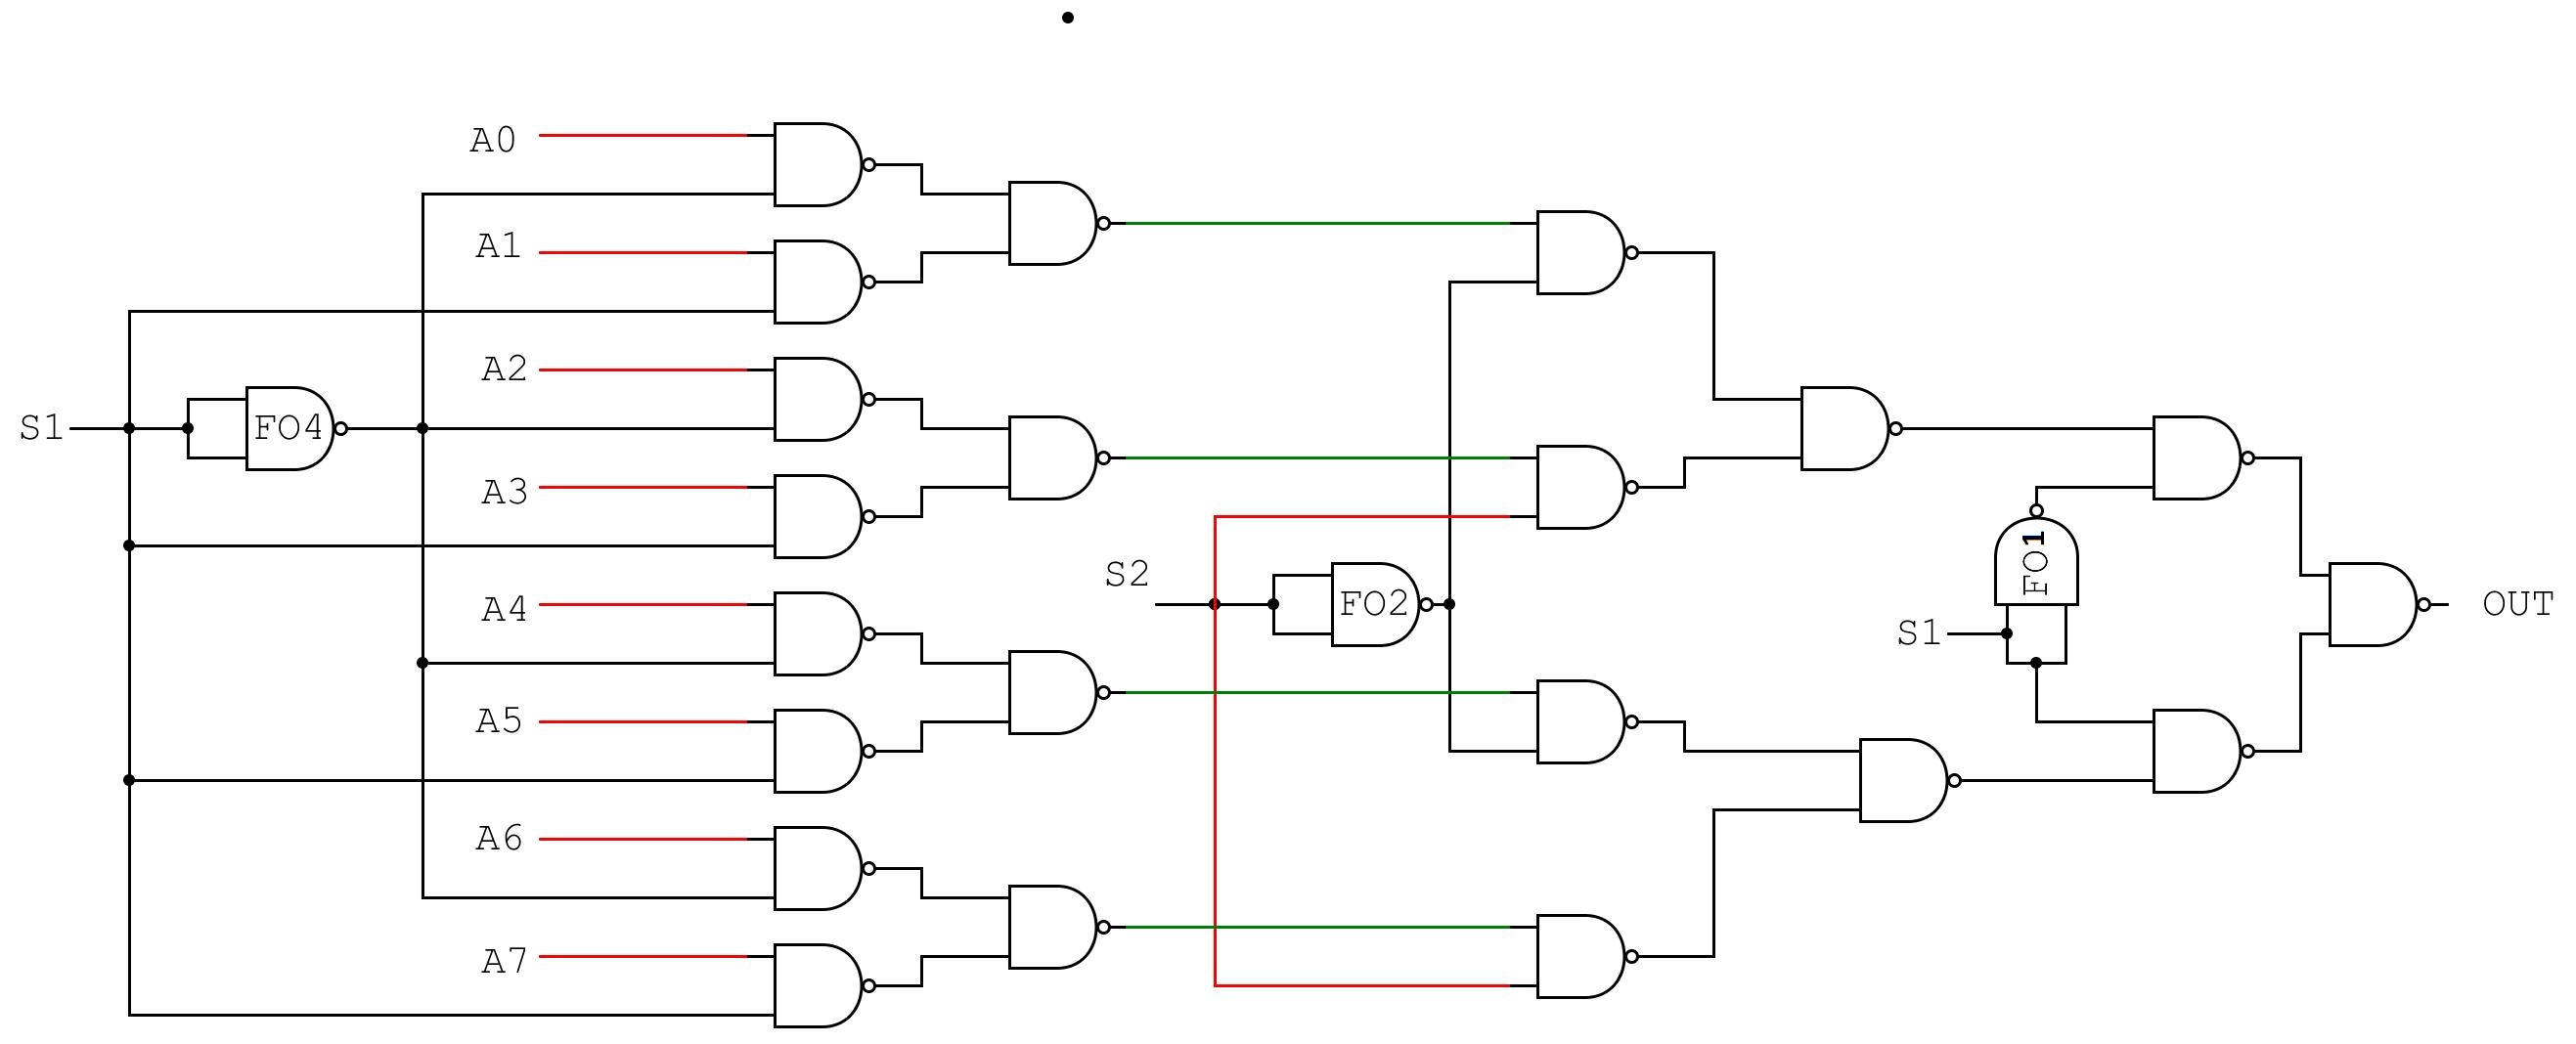
\includegraphics[scale=0.15]{immagini/8_to_1_1bit}
	\caption{\textit{Circuit implementation of a  multiplexer 8 to 1 with only NAND gates.}} 
	\label{8_to_1_1bit}
\end{figure}
\newpage
\section{CMOS realization of multiplexers} 
The next step is to realize a MUX circuit with transistors, by implementing CMOS technology. The building unit is reported in figure \ref{nand2} where a NAND gate is showed.
\begin{figure}[!h]
	\centering
	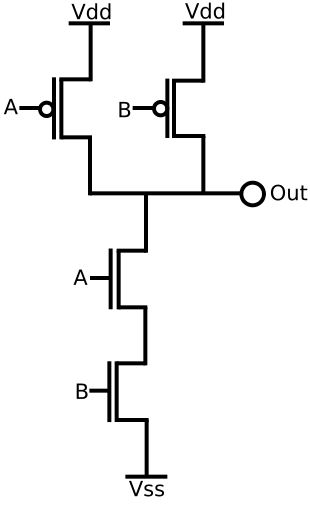
\includegraphics[scale=0.3]{immagini/nand2.png}
	\caption{\textit{CMOS circuit for a NAND gate.}} 
	\label{nand2}
\end{figure}
\newline
An example of CMOS multiplexer realization is reported in the figure below.
\begin{figure}[!h]
	\centering
	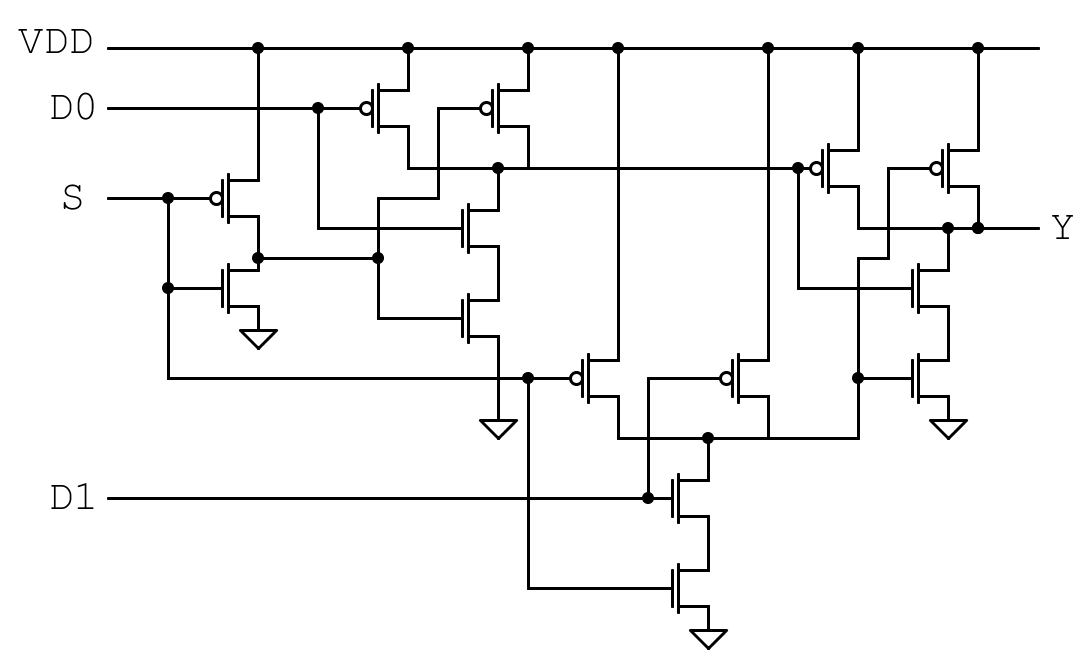
\includegraphics[scale=0.4]{immagini/trans}
	\caption{\textit{CMOS realization of a MUX 2x1.}} 
	\label{mux_3}
\end{figure}


\newpage
\section{Types of Multiplexer}
Here are summarized the different typologies of mutiplexer analysed. The various multiplexers vary by the number of input signals and the parallelism. 
\begin{itemize}\itemsep1pt
	\item Multiplexer 2 to 1 parallelism 16 bit
	\item Multiplexer 2 to 1 parallelism 32 bit
	\item Multiplexer 2 to 1 parallelism 64 bit 
	\item Multiplexer 8 to 1 parallelism 8 bit 	
	\item Multiplexer 16 to 1 parallelism 8 bit
	\item Multiplexer 16 to 1 parallelism 16 bit
	\item Multiplexer 16 to 1 parallelism 32 bit
	\item Multiplexer 16 to 1 parallelism 64 bit 
	\item Multiplexer 32 to 1 parallelism 8 bit
	\item Multiplexer 32 to 1 parallelism 16 bit
	\item Multiplexer 32 to 1 parallelism 32 bit
	\item Multiplexer 32 to 1 parallelism 64 bit 
	\item Multiplexer 64 to 1 parallelism 8 bit
	\item Multiplexer 64 to 1 parallelism 16 bit
	\item Multiplexer 64 to 1 parallelism 32 bit
	\item Multiplexer 64 to 1 parallelism 64 bit 
	\item Multiplexer 128 to 1 parallelism 8 bit
	\item Multiplexer 128 to 1 parallelism 16 bit
	\item Multiplexer 128 to 1 parallelism 32 bit
	\item Multiplexer 128 to 1 parallelism 64 bit 
\end{itemize}

	\chapter{Power consumption}
In this chapter are presented the calculations performed for the power consumption in CMOS multiplexers. By using the application TAMTAMS web, it was possible to make a first analysis at system level of several parameters concerning CMOS NAND2 gates employed.  
\section{Theoretical analysis}
\paragraph{Static Power}
is generated by the contribution of two different leakage currents: subthreshold current and gate current.
Static power is considered as the product between the supply voltage $\left( V_{dd} \right)$  and the leakage currents probabilistic mean value.
\\
\paragraph{Dynamic Power}
is described by the following expression
\begin{equation*}
P_{DYN}= f_{ck} V_{DD}^{2} E_{SW} C_{L},
\end{equation*}
where contributes are:
	\begin{description}
		\item[$V_{DD}$] voltage supply. Dynamic power consumption has a quadratic relation with it, so to reach a further power dissipation decreasing we should act on it;
		\item[$f_{ck}$] clock frequency. Faster is the device behaviour, higher is the consumption;
		\item[$E_{SW}$] switching activity. It is the number of transition per period;
		\item[$C_{L}$] load capacitance. Is the load that the device has to drive.
	\end{description}
To compute the dynamic power consumption, the basic MUX unit has been studied and the worst case has been selected: the maximum switching activity has been obtained analyzing the following truth table where the starting configuration is assumed as $A=B=0$ and $S=1$:
	\begin{table}[h]
	\centering
	\caption{Truth table for transition analysis}
	\label{my-label}
		\begin{tabular}{lllll}
		\textbf{A} & \textbf{B} & \textbf{S} & \textbf{Y} & \textbf{Transitions} \\
		0          & 0          & 0          & 0          & 1                    \\
		0          & 0          & 1          & 0          & 0                    \\
		0          & 1          & 0          & 0          & 2                    \\
		0          & 1          & 1          & 1          & 2                    \\
		1          & 0          & 0          & 1          & 3                    \\
		1          & 0          & 1          & 0          & 0                    \\
		1          & 1          & 0          & 1          & 3                    \\
		1          & 1          & 1          & 1          & 2                   
		\end{tabular}
	\end{table}

%%TODOOOOOOOOOOOOOOOOOOOOOOOOOOOOOOOOOOOOOOOOOOOOOOOOOOOOOOOOOOOOOOOOOOOOOOO	

We have maximum switching activity when $A=1$, $B$ doesn't care, $S=0$. This configuration determines that three gates (2 NAND2 and 1 inverter) output commute at the same time (see figure \ref{fig:2_to_1_1bit_dyn}). 
In order to compute the dynamic power consumption we have taken into account only the worst case condition, considering for every elementary mux structure the consumption associated to the commutation of 2 NAND2 and 1 inverter.
	\begin{figure}[h]
		\centering
		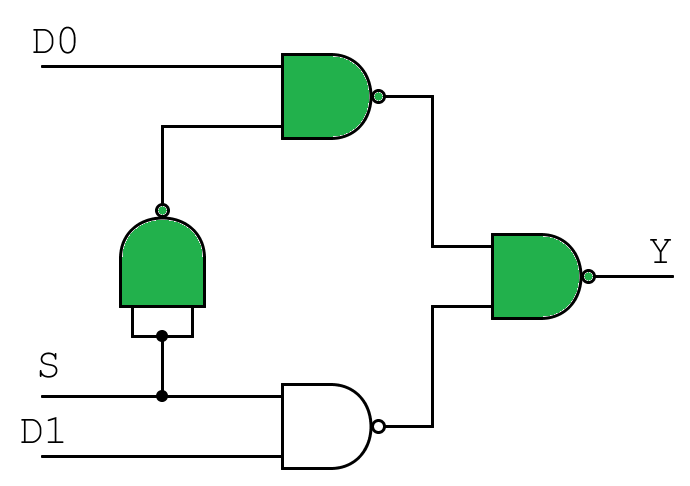
\includegraphics[width=0.5\textwidth]{immagini/2_to_1_1bit_dyn.png}
		\caption{Basic MUX structure. In green are represented gates defining the maximum switching activity.}
		\label{fig:2_to_1_1bit_dyn}
	\end{figure}
%---------------------------------------------------------------
%	MODELLI
%---------------------------------------------------------------
\subsection{Models}
Here is presented the models employed in the power evaluation. To represent the characteristics of each mux circuit, we used the following notation:  
	\begin{description}
		\item[$X$]	stands for configuration number input;	%numero di input della configurazione
		\item[$W$]	describes the parallelism, number of bit, that compose a single mux input information.
	\end{description}
\paragraph{Static power model}
To compute the total amount of static power, it is necessary to consider the single NAND2 static power consumption, obtained with TAMTAMS analysis. This value has to be multiplied by the total number of gates in the configuration under exam. For instance,a basic 2-to-1 mux with $W=1$, is obtained from a total amount of 4 NAND2 gates  with fan out of 1 (FO1), according to figure \ref{fig:2_to_1_1bit_dyn}. Generalizing for a mux with number of input $X$ and parallelism $W$, it is possible to express a general equation describing the amount $N_{gates}$ of NAND2 needed.
\begin{equation}
N_{gates} = \underbrace{3 W \left( X-1 \right)}_\text{number of NAND2} \ \ \ \ \ \ \  + \underbrace{\frac{W}{4}\left( X-1\right) .}_\text{number of NAND2 to build inverters}
\label{magic}
\end{equation}
Moreover, the term expressing the number of NAND inverter, gives information about the fan-out of inverters in the circuit. Let's see three examples of how this equation work.
\textbf{Example 1}\\
Consider a mux 4-to-1 with W=2.\\
The amount of logic NAND2 needed are:  $3 W \left( X-1 \right) = 18. $
The amount of NAND2 inverters are: $W/4\left( X-1\right) = 1.5=  \underbrace{1}_\text{one NAND2 FO4} + \underbrace{0.5}_\text{one NAND2 FO2}$\\
\textbf{Example 2}\\
Consider a mux 8-to-1 with W=2.\\
The amount of logic NAND2 needed are:  $3 W \left( X-1 \right) = 42. $
The amount of NAND2 inverters are: $W/4\left( X-1\right) = 3.5=  \underbrace{3}_\text{tree NAND2 FO4} + \underbrace{0.5}_\text{one NAND2 FO2}$\\
\textbf{Example 3}\\
Consider a mux 8-to-1 with W=1.\\
The amount of logic NAND2 needed are:  $3 W \left( X-1 \right) = 21. $
The amount of NAND2 inverters are: $W/4\left( X-1\right) = 1.75=  \underbrace{1}_\text{one NAND2 FO4} + \underbrace{0.5}_\text{one NAND2 FO2}+  \underbrace{0.25}_\text{one NAND2 FO1}$\\
In the end, to obtain the power values for static consumptions, numbers obtained with this model have been multiplied with the NAND2 static power dissipation values taken from TAMTAMS analysis.

\paragraph{Dynamic power model}
From considerations derived from the truth table with the analysis of transitions in a single 2-to-1 mux, presented at the beginning of this chapter, the mathematical expression representing maximum number of gate commutations in a generic X-to-1 mux with parallelism $W$ is 
\begin{equation}
N_{transitions} = \underbrace{2 W \left( X-1 \right)}_\text{wort case NAND2 transitions}   + \underbrace{\frac{W}{4}\left( X-1\right) .}_\text{wort case inverter transitions}
\end{equation}
As always, the term expressing the number of NAND inverter, gives information about the fan-out of inverters commuting in the circuit.
In order to  obtain the power values for the dynamic consumptions, numbers obtained with this model have been multiplied with the NAND2 dynamic power dissipation values taken from TAMTAMS analysis.
\newpage

\section{Simulation results}
\begin{table}[b!]
\centering
\label{my-label}
\begin{tabular}{@{}llllllll@{}}
\toprule
\multicolumn{2}{l}{\textbf{Configuration}} & \multicolumn{2}{l}{\textbf{HP\_2010}} & \multicolumn{2}{l}{\textbf{LOP\_2010}} & \multicolumn{2}{l}{\textbf{LSTP\_2010}} \\ \midrule
\textit{Input}         & \textit{Word}        & \textit{Static}   & \textit{Dynamic}  & \textit{Static}   & \textit{Dynamic}   & \textit{Static}    & \textit{Dynamic}   \\
2                      & 1                 & 0.00081W           & 7.133e-6W          & 8.076e-6 W         & 2.717e-6W           & 4.609e-7W           & 3.927e-6W          
\end{tabular}
\end{table}

%2to1 Wx
% Please add the following required packages to your document preamble:
% \usepackage{booktabs}
\begin{table}[b!]
\centering

\label{my-label}
\begin{tabular}{@{}llllllll@{}}
\toprule
\multicolumn{2}{l}{\textbf{Configuration}} & \multicolumn{2}{l}{\textbf{HP\_2010}} & \multicolumn{2}{l}{\textbf{LOP\_2010}} & \multicolumn{2}{l}{\textbf{LSTP\_2010}} \\ \midrule
\textit{Input}         & \textit{Word}        & \textit{Static}   & \textit{Dynamic}  & \textit{Static}   & \textit{Dynamic}   & \textit{Static}    & \textit{Dynamic}   \\
2                      & 8                 & 0.00524W           & 4.231e-5W          & 5.207e-5W          & 1.612e-5W           & 2.970e-6W          & 2.343e-5W           \\
2                      & 16                & 0.0105W            & 8.462e-5W          & 0.00010W           & 3.224e-5W           & 5.940e-6W           & 4.686e-5W           \\
2                      & 32                & 0.02097W           & 0.00017W           & 0.00021W           & 6.448e-5W           & 1.188e-5W           & 9.373e-5W           \\
2                      & 64                & 0.04194W          & 0.00034W           & 0.00042W           & 0.00013W            & 2.376e-5W           & 0.00019W           
\end{tabular}
\end{table}

%xto1 Wx
% input 16
\begin{table}[b!]
\centering
\label{my-label}
\begin{tabular}{@{}llllllll@{}}
\toprule
\multicolumn{2}{l}{\textbf{Configuration}} & \multicolumn{2}{l}{\textbf{HP\_2010}} & \multicolumn{2}{l}{\textbf{LOP\_2010}} & \multicolumn{2}{l}{\textbf{LSTP\_2010}} \\ \midrule
\textit{Input}         & \textit{Word}        & \textit{Static}   & \textit{Dynamic}  & \textit{Static}   & \textit{Dynamic}   & \textit{Static}    & \textit{Dynamic}   \\
16                     & 8                 & 0.0786W            & 0.0006W            & 0.0008W            & 0.0002W             & 4.455e-5W           & 0.0003W             \\
16                     & 16                & 0.1573W            & 0.0013W            & 0.0016W            & 0.0005W             & 8.9106e-5W          & 0.0007W             \\
16                     & 32                & 0.3145W            & 0.0025W            & 0.0031W            & 0.0010W             & 0.0002W             & 0.0014W             \\
16                     & 64                & 0.6290W            & 0.0051W            & 0.0062W            & 0.0019W             & 0.0004W             & 0.0028W            
\end{tabular}
\end{table}
% input 32
\begin{table}[b!]
\centering
\label{my-label}
\begin{tabular}{@{}llllllll@{}}
\toprule
\multicolumn{2}{l}{\textbf{Configuration}} & \multicolumn{2}{l}{\textbf{HP\_2010}} & \multicolumn{2}{l}{\textbf{LOP\_2010}} & \multicolumn{2}{l}{\textbf{LSTP\_2010}} \\ \midrule
\textit{Input}         & \textit{Word}        & \textit{Static}   & \textit{Dynamic}  & \textit{Static}   & \textit{Dynamic}   & \textit{Static}    & \textit{Dynamic}   \\
32                     & 8                 & 0.1625W            & 0.0013W            & 0.0016W            & 0.0005W             & 9.208e-5W           & 0.0007W             \\
32                     & 16                & 0.3250W            & 0.0026W            & 0.0032W            & 0.0010W             & 0.0002W             & 0.0015W             \\
32                     & 32                & 0.6500W            & 0.0052W            & 0.0065W            & 0.0020W             & 0.0004W             & 0.0029W             \\
32                     & 64                & 1.3000W            & 0.0105W            & 0.0129W            & 0.0040W             & 0.0007W             & 0.0058W            
\end{tabular}
\end{table}
% input 64
\begin{table}[b!]
\centering
\label{my-label}
\begin{tabular}{@{}llllllll@{}}
\toprule
\multicolumn{2}{l}{\textbf{Configuration}} & \multicolumn{2}{l}{\textbf{HP\_2010}} & \multicolumn{2}{l}{\textbf{LOP\_2010}} & \multicolumn{2}{l}{\textbf{LSTP\_2010}} \\ \midrule
\textit{Input}         & \textit{Word}        & \textit{Static}   & \textit{Dynamic}  & \textit{Static}   & \textit{Dynamic}   & \textit{Static}    & \textit{Dynamic}   \\
64                     & 8                 & 0.3302W            & 0.0027W            & 0.0033W            & 0.0010W             & 0.0002W             & 0.0015W             \\
64                     & 16                & 0.6605W            & 0.0053W            & 0.0066W            & 0.0020W             & 0.0004W             & 0.0029W             \\
64                     & 32                & 1.3210W            & 0.0107W            & 0.0131W            & 0.0041W             & 0.0007W             & 0.0059W             \\
64                     & 64                & 2.6420W            & 0.0213W            & 0.0262W            & 0.0081W             & 0.0015W             & 0.01181W           
\end{tabular}
\end{table}
% input 128

\begin{table}[b!]
\centering
\label{my-label}
\begin{tabular}{@{}llllllll@{}}
\toprule
\multicolumn{2}{l}{\textbf{Configuration}} & \multicolumn{2}{l}{\textbf{HP\_2010}} & \multicolumn{2}{l}{\textbf{LOP\_2010}} & \multicolumn{2}{l}{\textbf{LSTP\_2010}} \\ \midrule
\textit{Input}         & \textit{Word}        & \textit{Static}   & \textit{Dynamic}  & \textit{Static}   & \textit{Dynamic}   & \textit{Static}    & \textit{Dynamic}   \\
128                    & 8                 & 0.6657W            & 0.0054W            & 0.0066W            & 0.0020W             & 0.0004W             & 0.0030W             \\
128                    & 16                & 1.3315W            & 0.0107W            & 0.0132W            & 0.0041W             & 0.0007W             & 0.0060W             \\
128                    & 32                & 2.6630W            & 0.0215W            & 0.0264W            & 0.0082W             & 0.0015W             & 0.0119W             \\
128                    & 64                & 5.3259W            & 0.0430W            & 0.0529W            & 0.0164W             & 0.0030W             & 0.0238W            
\end{tabular}
\end{table}

\newpage
%---------------------------------------------------------------
%	DISCUSSIONE
%---------------------------------------------------------------
\section{Discussion}
\textbf{Static Power}:
\textit{HP} technology has high static power value consumption due to the necessity to reach faster commutation speed compared to the others.\\
\textit{LSTP} technology, instead, has can be seen from the results, has been designed to reach the opposite situation (lowest static power consumption).\\
In the end, \textit{LOP} technology is a middle way solution because to reach lowest dynamic power consumption the commutation can't be quite fast and the threshold voltage can't be so high (because it needs higher supply voltage).\\


\textbf{Dynamic Power}:
From the results can be seen that \textit{HP} technology reaches highest dynamic power consumption, this is due to their purpose to achieve the fastest commutation velocity.\\
\textit{LOP} technology results shows that the theoretical assumption is correct, so its values are the lowest ones.\\
\textit{LSTP} technology is a middle way solution because to activate the gate the supply voltage needed is the higher one, due to its higher threshold voltage.\\

\begin{figure}[!h]
	\centering
	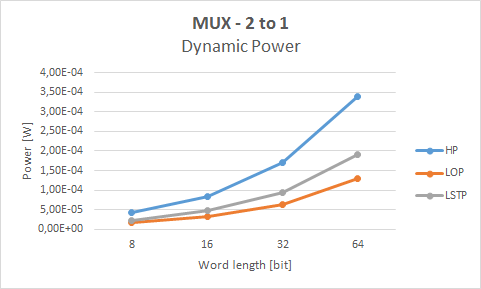
\includegraphics[scale=0.8]{immagini/2to1D}
	\caption{\textit{}} 
	\label{1}
\end{figure}
\newpage
\begin{figure}[!h]
	\centering
	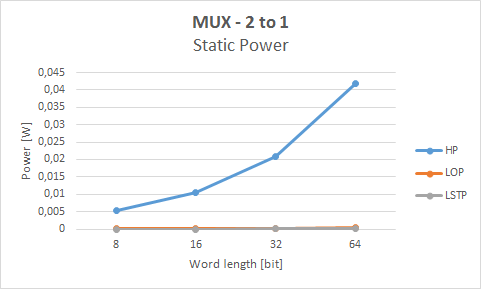
\includegraphics[scale=0.8]{immagini/2to1S}
	\caption{\textit{}} 
	\label{2}
\end{figure}

\begin{figure}[!h]
	\centering
	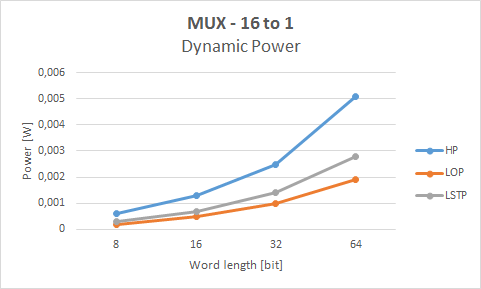
\includegraphics[scale=0.8]{immagini/16to1D}
	\caption{\textit{}} 
	\label{3}
\end{figure}

\begin{figure}[!h]
	\centering
	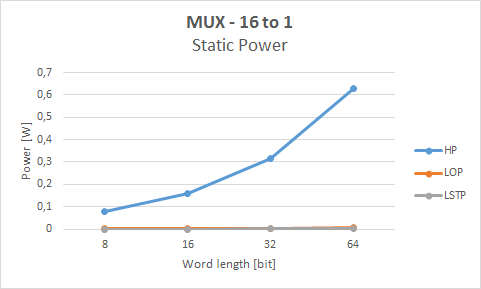
\includegraphics[scale=0.8]{immagini/16to1S}
	\caption{\textit{}} 
	\label{4}
\end{figure}
\newpage
\begin{figure}[!h]
	\centering
	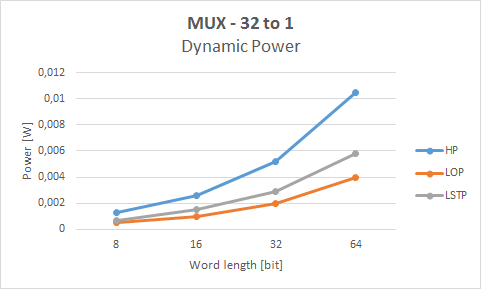
\includegraphics[scale=0.8]{immagini/32to1D}
	\caption{\textit{}} 
	\label{5}
\end{figure}

\begin{figure}[!h]
	\centering
	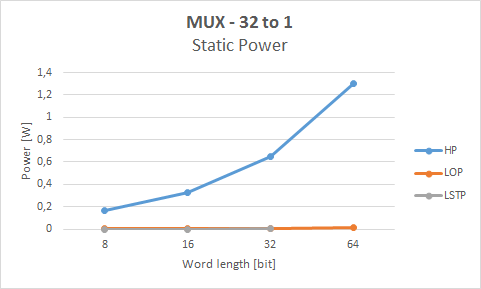
\includegraphics[scale=0.8]{immagini/32to1S}
	\caption{\textit{}} 
	\label{6}
\end{figure}

\begin{figure}[!h]
	\centering
	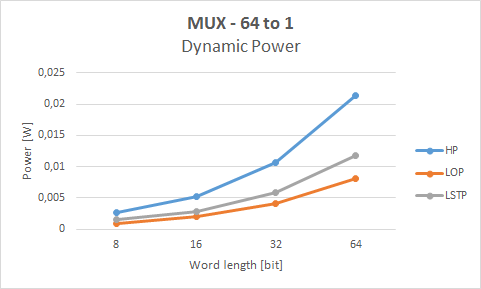
\includegraphics[scale=0.8]{immagini/64to1D}
	\caption{\textit{}} 
	\label{7}
\end{figure}
\newpage
\begin{figure}[!h]
	\centering
	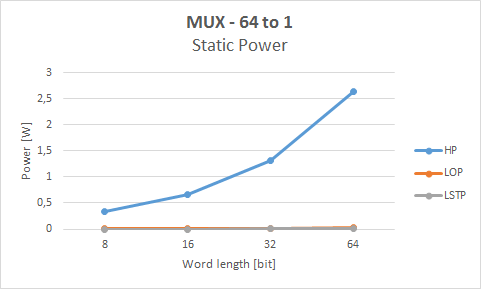
\includegraphics[scale=0.8]{immagini/64to1S}
	\caption{\textit{}} 
	\label{8}
\end{figure}

\begin{figure}[!h]
	\centering
	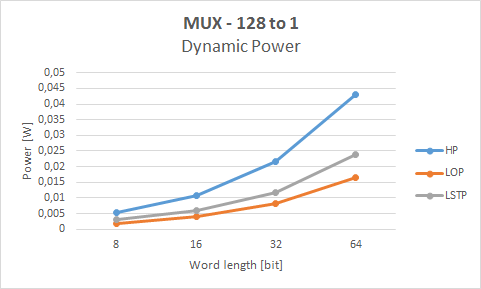
\includegraphics[scale=0.8]{immagini/128to1D}
	\caption{\textit{}} 
	\label{9}
\end{figure}

\begin{figure}[!h]
	\centering
	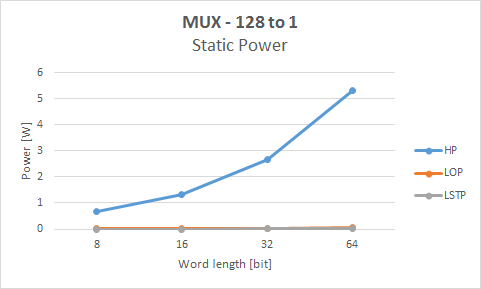
\includegraphics[scale=0.8]{immagini/128to1S}
	\caption{\textit{}} 
	\label{10}
\end{figure}
\newpage
%---------------------------------------------------------------
%	CODICE
%---------------------------------------------------------------
\section{Matlab implementation}
In the table below are reported the input data.

\begin{table}[h]
	\begin{center}
		\begin{tabular}{|c|c|c|c|} \hline
			\textbf{Quantity name} & \textbf{Description} & \textbf{u.m. (S.I.)} & \textbf{Variable name} \\ \hline
			$X$ &Number of input (is a power of 2) & / & X \\ 
			$W$ &Parallelism (is a power of 2) & / & Word \\
			$P_{static} NAND FO1$ &Static power NAND FO1 & W & P\_stat\_FO1 \\ 
			$P_{static} NAND FO2$ &Static power NAND FO2 & W & P\_stat\_FO2 \\ 
			$P_{static} NAND FO4$ &Static power NAND FO4 & W & P\_stat\_FO4 \\ 
			$P_{dyn} NAND FO1$ &Dynamic power NAND FO1 & W & P\_dyn\_FO1 \\ 
			$P_{dyn} NAND FO2$ &Dynamic power NAND FO2 & W & P\_dyn\_FO2 \\ 
			$P_{dyn} NAND FO4$ &Dynamic power NAND FO4 & W & P\_dyn\_FO4 \\  \hline 
		\end{tabular}
	\end{center}
	\caption{Input data}
	\label{tab1}
\end{table}

In the table below are reported the output data.

\begin{table}[h]
	\begin{center}
		\begin{tabular}{|c|c|c|c|} \hline
			\textbf{Quantity name} & \textbf{Description} & \textbf{u.m. (S.I.)} & \textbf{Variable name} \\ \hline
			$P_{static}$ &Static power MUX & W & P\_stat \\ 
			$P_{dynamic}$ &Dynamic power MUX & W & P\_dyn \\ \hline 
		\end{tabular}
	\end{center}
	\caption{Input data}
	\label{tab1}
\end{table}

\subsection{Main code}
The program asks the user to select the technology workspace needed and requires to specify the number of inputs and the parallelism of the MUX. The programs needs that both number of inputs and parallelism are power of two.
	\lstinputlisting{capitoli/code/main_mux_power.m}	
	
%\end{titlepage}


	\chapter{MUX time propagation delay }
In this chapter are presented the time delay calculations for all the previously showed multiplexers. Calculations have been performed using a "dividi et impera" approach, relying on the possibility to subdivide advanced multiplexer structures in  2-to-1 NAND2 based mux units. An RC delay model have been exploited, where the time constant of a single NAND gate is given by the total capacitance in the output node  times an effective resistance depending from the voltage source $V_{DD}$ and a ON current $I_{ON}$. In order to carry out quick estimations, we have considered a smart approach presented during lectures, referring on NAND2 statistical loads. Calculations have been done for CMOS MUX in HP, LOP and LSTP 2010 technologies.	

\section{Theoretical analysis}
According to the Roadmap, the average output of a NAND2 gate is fan-out of 4 made by inverters. It is therefore convenient to consider the total load capacitance of a NAND2 gate, as a sum of three different contributions
\begin{equation}
C_{ND2} = C_{FO4} + C_{metal} + C_J,
\end{equation}\\
where $C_{FO4}$ is an fan-out of 4 ideal statistical load, given by four inverters. The term $ C_{metal}$ accounts for capacitive contributions due to interconnects and $C_J$ accounts for junction capacitances. Overhead contributions of metallic interconnects and junctions have been estimated to be around 15\% of the ideal $C_{FO4}$.
It is possible to rewrite the previous expression in a more compact form
\begin{equation}
C_{ND2} = M \ C_{FO4},
\end{equation}
where $M$ has been fixed to  $1.5$ and plays the role of parasitic multiplier. According to theory,  $C_{FO4}$ is given by four times the value assumed by a simpler $C_{FO1}$ that can be written as $C_{FO1} = C_{gate_n}\ (1 + W_p/W_n) = 2.29 \  C_{gate_n}$. The nMOS gate capacitance can be expressed at first order by three different contributions involving the oxide capacitance, drain and source extension capacitances and a capacitance term modelling fringe effect. The capacitive contribution duo to the extensions has been considered 20\% of the oxide capacitance.  It is possible therefore to rewrite a plausible representation of the NAND2 load capacitance as a function of several CMOS technological parameters, taking into account all the three previously presented physical effects
\begin{equation}
C_{ND2} = 13.74 \left( \frac{\epsilon_{OX}}{t_{OX}} l_{ch} + 0.2 \frac{\epsilon_{OX}}{t_{OX}}  l_{ch} + C_{fringe}  \right) 
\end{equation}
Once the capacitances are known, it is necessary to evaluate the effective resistance. It can be represented as the ratio between the voltage source $V_{DD}$ and the ON current of a NAND2 gate ($I_{ND2_{ON}}$). In order to evaluate a worst-case situation, we consider the ON current of a NAND gate equal to the $I_{DS}$ current of a single pMOS transistor. This value has been evaluated using the Matlab MASTAR4 model reported in Tamtams. The effective resistance is given by the ratio $R = \frac{V_{DD}}{I_{ON}}$. The final value of the time constant of NAND2 gate is the simple RC product
\begin{equation}
\tau = R \ C_{ND2}.
\end{equation}

\subsection{MUX time delay}
The time delay evaluation in a multiplexer composed by a NAND tree structure follows simple rules.  In order to explain in a rigorous way the employed evaluation methodology, it is necessary to focus first the attention on a elementary block MUX 2x1. The critical path in a simple 2x1 mux is composed by three nand gates (see figure \ref{fig:mux2x1}) each one contributing for a unit of constant time. If we want to find the time delay of a 4x1 mux, it is necessary to consider a critical path defined by two 2x1 multiplexers connected in series. By extending this analysis to more advanced multiplexers, it is possible to write a generic expression for the total time delay, valid only in the simplified case of  multiplexers showing a nand tree structure
\begin{equation}
t = \tau \left[ 2 \log_2 (X) +1\right] 
\end{equation}
Where $X$ is the total number of input and is a power of two. Please notice that this general expression is unaffected by the parallelism $W$ of the system. In fact, increasing the parallelism will just affect the number of logic gates connected in parallel, without changing the critical path. Moreover, the simplicity of the expression is direct consequence of the choice to treat each nand gate in a statistical way, according to the roadmap recommendation.

\begin{figure}[!]
	\centering
	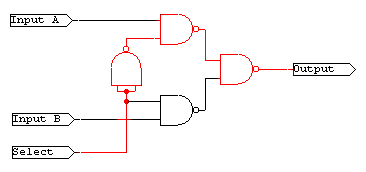
\includegraphics[scale =1]{capitoli/2x1}
	\caption{Representation of a 2x1 MUX. In red is highlighted the critical path.}
	\label{fig:mux2x1}
\end{figure}

\section{Simulation results}
Here are reported the time propagation delay numerical results of several multiplexers built according to the technologies HP, LSTP, LOP 2010. The simulations have been done for an arbitrary channel width $W_n = 270nm$. \\\\

\begin{tabular}{cccc}
	
	\cline{1-4}
	Number input    & HP & LOP & LSTP\\
	\hline
	2      & 35.58 ps    & 59.95 ps  &  59.96 ps  \\
	8  	  & 83 ps      & 130.6 ps    & 177.2ps  \\
	16       & 106.73 ps     & 167.9 ps    & 227.87 ps \\
	32       & 130.44 ps    & 205.15 ps     & 278.5 ps \\
	64 & 154.16 ps      & 242.44 ps      & 329.14 ps\\
	128 & 177.88 ps      & 279.74 ps     & 379.78 ps\\
	\hline
\end{tabular}
\\ \\
\subsection{Discussion}
In figure \ref{fig:time} are reported the simulation values together in a unique dispersion plot. As expected, the time delay of a high performance multiplexer shows smallest value with respect the other technologies. LSTP multiplexers are the slowest devices.
\begin{figure}[!]
	\centering
	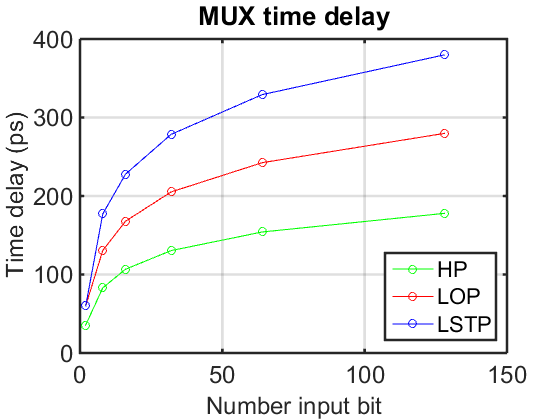
\includegraphics[scale =1]{capitoli/time}
	\caption{Time delay simulation results for 8, 16, 24, 32, 64, 128 inputs. Lines connecting each dot are just a graphical support.}
	\label{fig:time}
\end{figure}
\newpage

\section{Matlab implementation}
In the table below are reported the input data of the main script.

\begin{table}[h]
	\begin{center}
		\begin{tabular}{|c|c|c|c|} \hline
			\textbf{Quantity name} & \textbf{Description} & \textbf{u.m. (S.I.)} & \textbf{Variable name} \\ \hline
			$X$ &Number of input of MUX(is a power of 2) & / & X \\ 
			$C_{fringe}\ HP$ &Fringe capacitance MOS HP & F/nm & fring\_capHP2010 \\ 
			$C_{fringe} \ LOP$ &Fringe capacitance MOS LOP & F/nm & fring\_capLOP2010 \\ 
			$C_{fringe}\ LSTP$ &Fringe capacitance MOS LSTP & F/nm & fring\_capLSTP2010 \\
			$T_{ox}\ HP2010$ &Oxide thickness MOS HP2010 & nm & Tox\_HP2010 \\ 
			$T_{ox}\ LOP2010$ &Oxide thickness MOS LOP2010 & nm & Tox\_LOP2010 \\ 
			$T_{ox}\ LSTP2010$ &Oxide thickness MOS LSTP2010 & nm & Tox\_LSTP2010 \\
			$l_{ch}\ HP2010$ &channel length MOS HP2010 & nm & L\_HP2010 \\   
			$l_{ch}\ LOP2010$ &channel length MOS LOP2010 & nm & L\_LOP2010 \\
			$l_{ch}\ LSTP2010$ &channel length & nm & L\_LSTP2010 \\     
			$V_{DD}\ HP$ &Voltage source HP technology & V & Vdd\_HP2010 \\   
			$V_{DD}\ LOP$ &Voltage source LOP technology & V & Vdd\_LOP2010 \\ 
			$V_{DD}\ LSTP$ &Voltage source LSTP technology & V & Vdd\_LSTP2010 \\  \hline
		\end{tabular}
	\end{center}
	\caption{Input data}
	\label{tab1}
\end{table}

In the table below are reported the output data of the main script.

\begin{table}[h]
	\begin{center}
		\begin{tabular}{|c|c|c|c|} \hline
			\textbf{Quantity name} & \textbf{Description} & \textbf{u.m. (S.I.)} & \textbf{Variable name} \\ \hline
			$\tau \ HP2010$ &Time constant NAND2 HP2010 & s & Tsp\_HP\_nd2 \\
			$\tau \ LOP2010$ &Time constant NAND2 LOP2010 & s & Tsp\_LOP\_nd2 \\
			$\tau \ LSTP2010$ &Time constant NAND2 LSTP2010 & s & Tsp\_LSTP\_nd2 \\ 
			$t \ HP2010$ &Time delay mux HP2010 & s & tautotalHP \\
			$t \ LOP2010$ &Time delay mux LOP2010 & s & tautotalLOP \\
			$t \ LSTP2010$ &Time delay mux LSTP2010 & s & tautotalLSTP \\ \hline
		\end{tabular}
	\end{center}
	\caption{Output data}
	\label{tab1}
\end{table}
\subsection{Main time delay}
\begin{lstlisting}
%%%%%%%%%%%%%%%%%%%%%%%%%%%%%%%%%%%%%%%%%%%%%%%%%%%%
%                 MAIN Nand2 time delay                      
%%%%%%%%%%%%%%%%%%%%%%%%%%%%%%%%%%%%%%%%%%%%%%%%%%%%

clear all
close all

%Permittivity
eps_0 = 8.854187e-12 *1e-9; %F/nm
eps_SiO2 = 3.9*eps_0; %F/nm

%Fringe capacitances
fring_capHP2010 = 1.5e-16*1e-3; %F/nm
fring_capLOP2010 = 2.2e-16*1e-3;
fring_capLSTP2010 = 2.4e-16*1e-3;

%Oxide thickness
Tox_HP2010 = 0.65; %nm
Tox_LOP2010 = 0.9;
Tox_LSTP2010 = 1.4;

%Channel length
L_HP2010 = 18; %nm
L_LOP2010 = 22;
L_LSTP2010 = 28;

%Voltage source
VDD_HP2010 = 1; %V
VDD_LOP2010 = 0.7;
VDD_LSTP2010 = 1.1;

prompt = 'Specify the nMOS channel width Wn (nm):  ';
Wn = input(prompt)

%Total capacitance on output node of the Nand2 gate
C_nd2_HP = 13.74*(eps_SiO2*L_HP2010/Tox_HP2010 + fring_capHP2010 + ...
 0.2*eps_SiO2*L_HP2010/Tox_HP2010)*Wn;
C_nd2_LOP = 13.74*(eps_SiO2*L_LOP2010/Tox_LOP2010+fring_capLOP2010+ ...
0.2*eps_SiO2*L_LOP2010/Tox_LOP2010)*Wn;
C_nd2_LSTP=13.74*(eps_SiO2*L_LSTP2010/Tox_LSTP2010+fring_capLSTP2010 + ...
0.2*eps_SiO2*L_LSTP2010/Tox_LSTP2010)*Wn;

%Mastar model implementation
[Vth_nHP,Vth_pHP, Ioff_nHP, Ioff_pHP, Igate_nHP,...
Igate_pHP]= Mastar4_Vth_Ioff_IgHP2010();
[I_nMOSHP, I_pMOSHP]= Ion_Mastar_modelHP2010(Vth_nHP); %uA/um

[Vth_nLOP,Vth_pLOP, Ioff_nLOP, Ioff_pLOP, ...
Igate_nLOP, Igate_pLOP]= Mastar4_Vth_Ioff_IgLOP2010();
[I_nMOSLOP, I_pMOSLOP]= Ion_Mastar_modelLOP2010(Vth_nLOP); %uA/um

[Vth_nLSTP,Vth_pLSTP, Ioff_nLSTP, Ioff_pLSTP, ...
Igate_nLSTP, Igate_pLSTP]= Mastar4_Vth_Ioff_IgLSTP2010();
[I_nMOSLSTP, I_pMOSLSTP]= Ion_Mastar_modelLSTP2010(Vth_nLSTP); %uA/um

%NAND2 delay evaluation
Wp = 1.29*Wn;
Tdp_HP_nd2 =C_nd2_HP*VDD_HP2010/(I_pMOSHP*Wp*1e-3*1e-6); %s
Tdp_LOP_nd2 =C_nd2_LOP*VDD_LOP2010/(I_pMOSLOP*Wp*1e-3*1e-6); %s
Tdp_LSTP_nd2 =C_nd2_LSTP*VDD_LSTP2010/(I_pMOSLSTP*Wp*1e-3*1e-6); %s

prompt = 'Specify the number of channel inputs:  ';

X = input(prompt);
%Ninput has a mean only if is 2,4,8,16,32,64

%Time delay evaluation, s
tautotalHP =log2(X)*2*Tdp_HP_nd2+Tdp_HP_nd2 %s
tautotalLOP =log2(X)*2*Tdp_LOP_nd2+Tdp_LOP_nd2 %s
tautotalLSTP =log2(X)*2*Tdp_LSTP_nd2+Tdp_LSTP_nd2 %s
\end{lstlisting}

\subsection{Mastar4 Vth Ioff Ig HP2010()}
This is a function needed in order to evaluate the threshold voltages, the off and the gate current of MOS transistors.
The most part of the code has been taken from the Matlab modules of TAMTAMS.

\begin{lstlisting}
function [Vth_n,Vth_p, Ioff_n, Ioff_p, Igate_n,...
Igate_p]= Mastar4_Vth_Ioff_IgHP2010()
%Please see: https://tamtams.vlsilab.polito.it/...
%Documentation/TechnologyHTML/bulk/HP2010_dev_bul.html

%PARAMETERS           
%Please, select "Model" value for the technology type
%BULK = 0; FINFET = 1; SOI = 2; GAA = 3; CNT = 4;
Model = 0; 

%Physical parameters
q = 1.6021766208e-19;     % elementary charge (C)
kB = 1.3806488e-23;       % Boltzmann constant (J/K)
hbar = 1.054571800e-34;   % reduced Planck cons tant (Js)
m0 = 9.10938291e-31;      % electron mass (kg)
clight = 2.99792458e8 ;   % speed of light (m/s)
mu0 = (4* pi )*1e-7;      % vacuum magnetic permeability (H/m)
e0 = 1e-2/( clight ^2* mu0 );% vacuum electric permittivity (F/cm)
es = 11.8;                % Silicon relative dielectric constant
esio2 = 3.9;              % Silicon oxide relative dielectric constant
Eg0 = 1.166;              % Silicon energy gap at 300K (eV)
Alpha = 4.73e-4; Beta = 636;
Temp = 300;               % Absolute working temperature (K)
Eg = Eg0 - Alpha * Temp^2/(Temp + Beta);%Silicon energy gap (eV)
Vt = kB.*Temp./q;         %Termal voltage (V)
ni = sqrt(5.85e31*Temp^3*exp(-Eg/Vt));%Intrinsic carrier concentration(cm^-3)
Xs = 4.003;               % Silicon affinity (eV)

%Geometrical parameters (HP 2012)
Lgate =18; %nm, The effective length of the gate.
Xj = 6.5; %nm, Source/Drain extensions length.
LDDW = 50; %nm, Doping width of source/drain extension, value used only...
%for transistors image generation.
Tox = 0.65; %nm, Physical gate oxide thickness.
Darks = 0.27; %nm, 2.5 A=0.1nm Dark space length, used in...
%Mastar threshold voltage model.
Polyd = 0; %Poly depletion length, used in Mastar threshold voltage model.
Wt = 1000; %nm, Gate width of n-MOS.
beta =1.29; %is the ratio between Wp/Wn.
gateW_p = beta*Wt; %nm, Gate width of p-MOS
gateH = 40; %nm, Gate thickness, 
DopH = 30; %nm, Doping depth of source/drain
DopW = 100; %nm, Doping width of source/drain
ContW = 30; %nm, Contact width
Diff_ray = 5;%nm, Ray of annealing diffusion
Angle = 25; %deg, Pocket implantation angle

%Doping parameters (HP 2010)
Nbulk = 7.14e18; %cm^-3, Channel Doping
n_sub = 3.2e18; %cm^-3, Substrate Doping
n_plus_poly = 1e20; %cm^-3, Polysilicon n+ doping
Next = 7.819e18; %cm^-3, Extensions doping
n_source_drain = 1e20; %cm^-3, Source/Drain doping

%Electrical parameters (HP 2010)
rconst_n = 254.61; %Ohm, N-MOS access resistance
rconst_p = 254.61; %Ohm, P-MOS access resistance
Fring_cap = 1.5e-16; %F/um, Fringe capacitance per unit length
Ith = 5e-7; %A, Id at the threshold voltage (Vth_off)
Phi_m = 4.15; %V Built-in potential
Kfield = 1; %Effective electric field reduction

%Scaling factors (HP 2010)
Gamma = 0.7; % Scaling factor for lateral diffusion
Zeta = 0.8; %Scaling factor for drain induced lowering barrier (DIBL)
Zeta2 = 0.64; %Scaling factor for short channel effect (SCE)

%Power supply parameters (HP 2010)
Vdd = 1; %V Operation voltage (gate and drain voltages)

%Other parameters(HP 2010)
Cpoches = 5.2e13;
Rp = 10; %nm
Delta_rp = 6; %nm
Delta_rl = 3; %nm
ActivePkt = 0;


%THRESHOLD VOLTAGE, MASTAR 4 MODEL
% https://tamtams.vlsilab.polito.it/Documentation/ ...
ModulesHTML/vth/vth_mas_complete_bul.html

ni_temp = ni /3.79; %Fitting from Mastar
Phi_f = Vt*log(Nbulk/ni_temp); %Surface potential (V)
Vfb= Phi_m -(Xs + Eg/2 + Phi_f);
Vbi=Vt*log(Nbulk*Next/ni_temp^2);
Qdep=sqrt(2*es*e0*q*Nbulk*(2*Phi_f));
Tox_el=Tox*3.9/esio2 + Darks/10 + Polyd/10; %nm, Electrical oxide thickness 
% %considering the effect of Dark Space and Polysilicon depletion
Cox=esio2*e0/(Tox_el*1e-7); %Oxide capacitance evaluation [F/cm^2]
Vtlong=Vfb+2*Phi_f+Qdep/Cox; %Long channel threshold voltage
Lel=Lgate-Gamma*Xj; %Channel electric length [nm]

%Depletion depth calculation:
Tdepbulk=1e7*Qdep/(q*Nbulk);
% for BULK transistors
if(Model==0)
Tdep=Tdepbulk;
% for Double Gate transistors
elseif(Model==1)
Tdep=Xj/2;
Xj=Xj/2;
% for SOI transistors
else if (Tdepbulk<Xj)
Tdep=Tdepbulk;
else
Tdep=Xj;
end
end

EI=(1+(Xj/Lel)^2)*Tox_el*Tdep/(Lel)^2;
% Short Channel Effect (SCE) [V]
SCE=es/esio2*Zeta2*Vbi*EI;
% Drain Induced Barrier Lowering (DIBL) [V]
DIBL=es/esio2*Zeta*EI*Vdd;
Vth=Vtlong-SCE-DIBL;
Vth_n = Vth;
Vth_p = -Vth;


%SUBTHRESHOLD CURRENT, MASTAR 4 MODEL
% https://tamtams.vlsilab.polito.it/Documentation/...
ModulesHTML/ioff/Ioff_mas4_bul.html


Npocket=0.5*(Cpoches/((Rp+2*Delta_rp)*10^-7)); 
Lpocket=(Rp+2*Delta_rp)*sin(Angle*pi/180)+ ...
2*Delta_rl*cos(Angle*pi/180)-(Gamma*Xj)/2;
Lel = Lgate - Gamma * Xj; %Electrical channel length [nm]
Lmin=min(Lel,Lpocket); %Effective channel length
Nch = Nbulk + 2 * Npocket * (Lmin/Lel); %Channel doping
if (ActivePkt==0)
Ith_new = Ith*Wt/Lel;
else
Ith_new = Ith*Wt/Lel* 8 * 10^8 * Nch^(-0.4865);
end;

Qdep = sqrt(2*es*e0*q*Nbulk*(2*Phi_f)); %Depletion charge evaluation

%Depletion depth calculation
Tdepbulk=1e7*Qdep/(q*Nbulk);
% for BULK transistors
if(Model==0)
Tdep=Tdepbulk;
% for Double Gate transistors
elseif(Model==1)
Tdep=Xj/2;
Xj=Xj/2;
% for SOI transistors
else if (Tdepbulk<Xj)
Tdep=Tdepbulk;
else
Tdep=Xj;
end
end

SS=Vt*log(10)*(1+((es/esio2)*Kfield*(Tox_el/Tdepbulk))); %V/dec
Ioff_n=Ith_new*10^(-Vth/SS)*10^9;  %nA/um
Ioff_p=Ith_new*10^(-Vth/SS)*10^9;  %nA/um


% GATE CURRENT, MASTAR 4 MODEL
% https://tamtams.vlsilab.polito.it/Documentation/...
ModulesHTML/igate/Igate_Mastar4_bul.html

%a, b, c, d parameters:
ag = 1.44e5;	% A/cm^2
bg = -4.02;		% V^-2
cg = 13.05;		% V^-1
dg = 1.17;		% Angstrom^-1

%Gate current density
Jgate_n = ag*exp(bg*Vdd^2 + cg*Vdd)*exp(-dg*Tox*10)*10;	% nA/um^2
Jgate_p = ag*exp(bg*Vdd^2 + cg*Vdd)*exp(-dg*Tox*10)*10;

Igate_n= Jgate_n*Lgate*1e-3; % [nA/um]
Igate_p= Jgate_p*Lgate*1e-3; % [nA/um]

if (Model==1)
Igate_n=2*Igate_n;
Igate_p=2*Igate_p;
end
return
\end{lstlisting}

The other two functions Mastar4\_Vth\_Ioff\_IgLOP2010() and Mastar4\_Vth\_Ioff\_IgLSTP2010() are not reported here, since they change just for what concern constants. For more details please see the original Matlab scripts.

\subsection{Ion Master model HP 2010()}
This is a function needed in order to evaluate the $I_{ON}$ of MOS transistors.
The most part of the code has been taken from the Matlab modules of TAMTAMS.

\begin{lstlisting}
function [Ion_n, Ion_p]= Ion_Mastar_modelHP2010(Vth)

% PARAMETERS                
%Please, select "Model" value for the technology type
%BULK = 0; FINFET = 1; SOI = 2; GAA = 3; CNT = 4;
Model = 0; 

%Physical parameters
q = 1.6021766208e-19;     % elementary charge (C)
kB = 1.3806488e-23;       % Boltzmann constant (J/K)
hbar = 1.054571800e-34;   % reduced Planck cons tant (Js)
m0 = 9.10938291e-31;      % electron mass (kg)
clight = 2.99792458e8 ;   % speed of light (m/s)
mu0 = (4* pi )*1e-7;      % vacuum magnetic permeability (H/m)
e0 = 1e-2/( clight ^2* mu0 ); % vacuum electric permittivity (F/cm)
es = 11.8;                % Silicon relative dielectric constant
esio2 = 3.9;              % Silicon oxide relative dielectric constant
Eg0 = 1.166;              % Silicon energy gap at 300K (eV)
Alpha = 4.73e-4; Beta = 636;
Temp = 300;                % Absolute working temperature (K)
Eg = Eg0 - Alpha * Temp^2/(Temp + Beta);%Silicon energy gap (eV)
Vt = kB.*Temp./q;          %Termal voltage (V)
ni = sqrt(5.85e31*Temp^3*exp(-Eg/Vt)); %Intrinsic carrier concentration(cm^-3)
Xs = 4.003;                % Silicon affinity (eV)

%Geometrical parameters (HP 2010)
Lgate =18; %nm, The effective length of the gate.
Xj = 6.5; %nm, Source/Drain extensions length.
LDDW = 50; %nm, Doping width of source/drain extension
Tox = 0.65; %nm, Physical gate oxide thickness.
Darks = 0.27; %nm, 2.5 A=0.1nm Dark space length
Polyd = 0; %Poly depletion length
Wt = 1000; %nm, Gate width of n-MOS.
beta =1.29; %is the ratio between Wp/Wn.
gateW_p = beta*Wt; %nm, Gate width of p-MOS
gateH = 40; %nm, Gate thickness
DopH = 30; %nm, Doping depth of source/drain
DopW = 100; %nm, Doping width of source/drain
ContW = 30; %nm, Contact width
Diff_ray = 5;%nm, Ray of annealing diffusion
Angle = 25; %deg, Pocket implantation angle

%Doping parameters (HP 2010)
Nbulk = 7.14e18; %cm^-3, Channel Doping
n_sub = 3.2e18; %cm^-3, Substrate Doping
n_plus_poly = 1e20; %cm^-3, Polysilicon n+ doping
Next = 7.819e18; %cm^-3, Extensions doping
n_source_drain = 1e20; %cm^-3, Source/Drain doping

%Electrical parameters (HP 2010)
rconst_n = 254.61; %Ohm, N-MOS access resistance
rconst_p = 254.61; %Ohm, P-MOS access resistance
Fring_cap = 1.5e-16; %F/um, Fringe capacitance per unit length
Ith = 5e-7; %A, Id at the threshold voltage (Vth_off)
Phi_m = 4.15; %V Built-in potential
Kfield = 1; %Effective electric field reduction

%Scaling factors (HP 2010)
Gamma = 0.7; % Scaling factor for lateral diffusion
Zeta = 0.8; %Scaling factor for drain induced lowering barrier (DIBL)
Zeta2 = 0.64; %Scaling factor for short channel effect (SCE)

%Power supply parameters (HP 2010)
Vdd = 1; %V Operation voltage (gate and drain voltages)

%Other parameters(HP 2010)
Cpoches = 5.2e13;
Rp = 10; %nm
Delta_rp = 6; %nm
Delta_rl = 3; %nm
ActivePkt = 0;

ni_temp = ni /3.79; %Fitting from Mastar
Phi_f = Vt*log(Nbulk/ni_temp); %Surface potential (V)
Vfb= Phi_m -(Xs + Eg/2 + Phi_f);
Vbi=Vt*log(Nbulk*Next/ni_temp^2);
Qdep=sqrt(2*es*e0*q*Nbulk*(2*Phi_f));
Tox_el=Tox*3.9/esio2 + Darks/10 + Polyd/10; %nm, Electrical oxide thickness
% %considering the effect of Dark Space and Polysilicon depletion
Cox=esio2*e0/(Tox_el*1e-7); %Oxide capacitance evaluation [F/cm^2]
Vtlong=Vfb+2*Phi_f+Qdep/Cox; %Long channel threshold voltage
Lel=Lgate-Gamma*Xj; %Channel electric length [nm]

%Depletion depth calculation:
Tdepbulk=1e7*Qdep/(q*Nbulk);
% for BULK transistors
Model = 0;
if(Model==0)
Tdep=Tdepbulk;
% for Double Gate transistors
elseif(Model==1)
Tdep=Xj/2;
Xj=Xj/2;
% for SOI transistors
else if (Tdepbulk<Xj)
Tdep=Tdepbulk;
else
Tdep=Xj;
end
end
Sigma = 1;
Gamma = 0.7;
Xj = 6.5; %nm
d=Sigma*q*Nbulk*Tdep/(2*Cox*(2*Phi_f))*1e-7;

%Electrical channel length [nm]
Lel = Lgate - Gamma * Xj;

%Evaluation of the value of E critic field for...
%the electrons and holes with the approximation of...
%saturation velocity of carriers
Kvs = 1.1;
vsat = 1e7; %cm/s
%Effective electric field
%https://tamtams.vlsilab.polito.it/Documentation/ModulesHTML/...
mobility/mobility_mas_bul.html
Kfield = 1;
Eeff_n=Kfield*(1e-6*(Vdd+Vth-2*(Vfb+2*Phi_f)))/(6*Tox_el*1e-7);
Eeff_p=Kfield*(1e-6*(Vdd+2*Vth-3*(Vfb+2*Phi_f)))/(9*Tox_el*1e-7);
%Mobility in normal conditions
muac_n=330*Eeff_n^(-0.3);
muac_p=90*Eeff_p^(-0.3);
%Mobility in high electric field conditions
musr_n=1450*Eeff_n^(-2.9);
musr_p=140*Eeff_p^(-1);
%Effective mobility calculation [cm2 V-1 s-1]
Kp = 1;
mueff_n=Kp*muac_n*musr_n/(muac_n+musr_n)
mueff_p=Kp*muac_p*musr_p/(muac_p+musr_p)

%Evaluation of the value of E critic field for the electrons and holes...
 with the approximation of saturation velocity of carriers
Ecrit_n=2*Kvs*vsat/mueff_n;
Ecrit_p=2*Kvs*vsat/mueff_p;
%Evaluation of Vdsat with approssimation of high field and body ...
linearization of the Qn charge
Vdsat_n=(1/(Lel*1e-7*Ecrit_n)+(1+d)/(Vdd-Vth))^-1;
Vdsat_p=(1/(Lel*1e-7*Ecrit_p)+(1+d)/(Vdd-Vth))^-1;

%Evaluation of the saturation current without the channel resistance
Idsat0_n=0.5*mueff_n*Cox*(Wt/Lel)*(Vdd-Vth)*Vdsat_n;
Idsat0_p=0.5*mueff_p*Cox*(Wt/Lel)*(Vdd-Vth)*Vdsat_p;

%Evaluation of the Ion current by adding the contribute of channel resistance
Rconst_n = 256.61; %Ohm
Rconst_p = 256.61; %N-MOS access resistance
Ion_n=Idsat0_n/(1+(2*Rconst_n*Idsat0_n/(Vdd-Vth))- ...
Rconst_n*Idsat0_n/(Vdd-Vth+Lel*1e-7*Ecrit_n*(1+d)))*1e6; %uA/um
Ion_p=Idsat0_p/(1+(2*Rconst_p*Idsat0_p/(Vdd-Vth))- ...
Rconst_p*Idsat0_p/(Vdd-Vth+Lel*1e-7*Ecrit_p*(1+d)))*1e6; %uA/um
\end{lstlisting}
The other two functions Ion\_Mastar\_modelLSTP2010(Vth) and Ion\_Mastar\_modelLOP2010(Vth) are not reported here, since they change just for what concern constants. For more details please see the original Matlab scripts.
	\chapter{Multiplexer area}
\section{Theoretical analysis}
The area of a single transistor is estimated as the product between the length (L) and the width (W).
The overall length $L$ is the sum of the the gate and the source and drain lengths. For the symmetry of the MOS structure, we can imagine that both source and drain lengths are equal and depend from the gate length according to arbitrary design rules $L_{S/D}= \lambda L_{gate}$. 
\begin{equation}
L = L_{gate} + 2 \ L_{S/D}.
\end{equation}
 The width is different between the two transistors, but the ratio remains always the same ($W_p / W_n =1.29$). In order to evaluate the occupied area of a mux, it is necessary to obtain first the area of a single Nand made with the CMOS technology. Another important aspect to take into account is the interconnections override that has been estimated to be the 15\% of the logic gate area ($I_O=0.15$).
As results, the area of a single Nand2 ($A_{ND2}$) is:
\begin{equation}
A_{ND2}=2L \ (Wn+Wp) (1+I_O)
\end{equation}
Once the occupied area of a single Nand2 is known, it is necessary to know the overall number of gates in the circuit. To do so, we can use the equation \ref{magic} in chapter 2, that allows to do a smart and full estimation of the number of gates in our system.

\section{Simulation results}
Here are reported several tables with the occupation area expressed in $\mu m^2$, for a nMOS with a channel width of 270nm. The program of course allows to make calculations for a customized value of channel width.
\subsubsection{Hp Technology}
\begin{tabular}{|c|c|c|c|c|c|c|}
	\hline
	& \bfseries2x1 & \bfseries8x1 & \bfseries16x1 & \bfseries32x1 & \bfseries64x1 & \bfseries128x1 \\
	\hline
	\hline
	\bfseries8 bit&1.9966&13.9763&29.9492&61.8950&125.7867&253.578\\
	\hline
	\bfseries16 bit&3.9932&27.9526&59.8984&123.7901&251.5734&507.1400 \\
	\hline
	\bfseries32 bit&7.9865&55.9052&119.7569&247.5802&503.1468&1014.3 \\
	\hline
	\bfseries64 bit&15.9729&111.8104&239.5937&495.1604&1006.3& 2028.6 \\
	\hline
\end{tabular} 
\subsubsection{Lop Technology}
\begin{tabular}{|c|c|c|c|c|c|c|}
	\hline
	& \bfseries2x1 & \bfseries8x1 & \bfseries16x1 & \bfseries32x1 & \bfseries64x1 & \bfseries128x1 \\
	\hline
	\hline
	\bfseries8 bit&2.4403&17.0821&36.6046&75.6495&153.7393&309.9189 \\
	\hline
	\bfseries16 bit&4.8806&34.1643&73.2092&151.2990&307.4786&619.8378\\
	\hline
	\bfseries32 bit&9.7612&68.3286&146.4184&302.5980&614.9572&1239.7\\
	\hline
	\bfseries64 bit&19.5225&136.6572&292.8368&605.1960&1229.9&2479.4\\
	\hline
\end{tabular} 
\subsubsection{Lstp Technology}
\begin{tabular}{|c|c|c|c|c|c|c|}
	\hline
	& \bfseries2x1 & \bfseries8x1 & \bfseries16x1 & \bfseries32x1 & \bfseries64x1 & \bfseries128x1 \\
	\hline
	\hline
	\bfseries8 bit&3.1058&21.7409&64.5877&96.2812&195.6682&394.4423 \\
	\hline
	\bfseries16 bit&6.2117&43.4818&93.1753&192.5424&391.3364&788.8845\\
	\hline
	\bfseries32 bit&12.4234&86.9634&186.3507&385.1247&782.6728&1577.8 \\
	\hline
	\bfseries64 bit&24.8468&173.9273&372.7013&770.2495&1565.3&3155.5\\
	\hline
\end{tabular} 

\section{Discussion}
As expected the occupied area shows a net tendency to increase as a function of the parallelism. However, the occupied area of a HP technology is generally smaller than the other technologies.  And the LSTP technology shows the greatest occupied area as a function of number of the parallelism.
\begin{figure}[!]
	\centering
	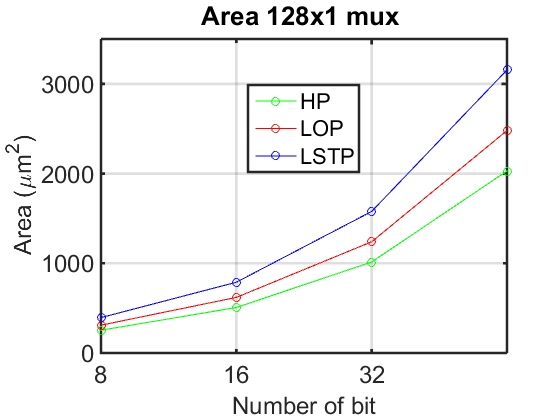
\includegraphics[scale =1]{capitoli/Area128to1}
	\caption{Occupied area of a mux 128x1 as a function of the parallelism}
	\label{fig:area}
	
\end{figure} 
\newpage

\section{Matlab implementation}
In the table below are reported the input data of the main script.

\begin{table}[h]
	\begin{center}
		\begin{tabular}{|c|c|c|c|} \hline
			\textbf{Quantity name} & \textbf{Description} & \textbf{u.m. (S.I.)} & \textbf{Variable name} \\ \hline
			$X$ &Number of input (is a power of 2) & / & X \\ 
			$W$ &Parallelism (is a power of 2) & / & Word \\
			$W_n$ &Gate width & um & Wn \\ 
			$I_O$ &Interconnections override & / &interc\_override \\ 
			$\lambda$ &design parameter to determine $L_{S/D}$ & / & lambda\\
			$L_{gate}$ &Gate length HP, LOP, LSTP 2010 & um & Lgate \\	 \hline
		\end{tabular}
	\end{center}
	\caption{Input data}
	\label{tabn}
\end{table}

In the table below are reported the output data of the main script.

\begin{table}[h]
	\begin{center}
		\begin{tabular}{|c|c|c|c|} \hline
			\textbf{Quantity name} & \textbf{Description} & \textbf{u.m. (S.I.)} & \textbf{Variable name} \\ \hline
			$A_{MUX} \ HP2010$ &Area MUX HP 2010 & $\mu m^2$ & AreaHP \\
			$A_{MUX} \ LOP2010$ &Area MUX LOP 2010 & $\mu m^2$ & AreaLOP \\
			$A_{MUX} \ LSTP2010$ &Area MUX LSTP 2010 & $\mu m^2$ & AreaLSTP \\  \hline
		\end{tabular}
	\end{center}
	\caption{Output data}
	\label{tabna}
\end{table}

\subsection{Main code}
\lstinputlisting{capitoli/main_area.m}
	
%\include{capitoli/3-Theory}
	%\include{capitoli/4-Simulation}
	%\include{capitoli/5-Results}
	%\include{capitoli/8-Bibliography}
	
	
	
\end{document}